\documentclass{article}

\usepackage{layouts}

\usepackage[utf8]{inputenc}
\usepackage[T1]{fontenc}
\usepackage{mathptmx}
\usepackage{amsmath}
\usepackage{graphicx}
\newcommand{\minus}{\scalebox{0.75}[1.0]{$-$}}
\usepackage{fancyhdr}
\usepackage{url}
\usepackage{xcolor}
\usepackage{hyperref}
\usepackage{csquotes}
%\usepackage{geometry}
\usepackage{emptypage}
\usepackage[parfill]{parskip} % removes indentation of sectioning.

% For tikz images
\usepackage{filecontents}
\usepackage{tikz}
\usepackage{graphicx}
\usepackage{caption}
\usepackage{subcaption}
\usepackage{amsmath}

\usetikzlibrary{arrows}
\usepackage{pgfplots}
\usetikzlibrary{calc,fadings,decorations.pathreplacing}

\usetikzlibrary{matrix,positioning,fit,backgrounds,intersections, fit, arrows.meta, shapes}

\usepackage{titlesec}

\setcounter{secnumdepth}{4} % gives numbers to subsubsections
\usepackage{hyperref}
\usepackage{graphicx}
\usepackage{multirow}
\usepackage[margin=0.9in]{geometry}
\usepackage[acronym, nonumberlist]{glossaries}
\makeglossaries
 
\usepackage[labelfont=bf]{caption} % Gives bold figure X. 
 
\usepackage{amsmath}

\usepackage[utf8]{inputenc}

\title{Machine Learning part of theoretical background}
\author{Hanna Svennevik}
\date{February 2020}

\begin{document}
\maketitle
%\begin{figure}[hp]
\centering
\def\layersep{2.5cm}
\begin{tikzpicture}[shorten >=1pt,->,draw=blue, node distance=\layersep]
    \tikzstyle{every pin edge}=[<-,shorten <=1pt]
    \tikzstyle{neuron}=[circle,fill=black!25,minimum size=17pt,inner sep=0pt]
    \tikzstyle{input neuron}=[neuron, fill=green];
    \tikzstyle{output neuron}=[neuron, fill=red];
    \tikzstyle{hidden neuron}=[neuron, fill=cyan];
    \tikzstyle{annot} = [text width=4em, text centered]

    \node[input neuron] (I-1) at (0,-1) {}; % {$T_{2m}$};
    \node[input neuron] (I-2) at (0,-2) {}; % {$q_v$};
    \node[input neuron] (I-3) at (0,-3) {}; % {$RH$};
    \node[input neuron] (I-4) at (0,-4) {}; % {$p_s$};

    % Draw the input layer nodes
    %\foreach \name / \y in {1,...,4}
    % This is the same as writing \foreach \name / \y in {1/1,2/2,3/3,4/4}
    %    \node[input neuron, pin=left:Input \#\y] (I-\name) at (0,-\y) {};

    % Draw the hidden layer nodes
    \foreach \name / \y in {1,...,5}
        \path[yshift=0.5cm]
            node[hidden neuron] (H-\name) at (\layersep,-\y cm) {};

    % Draw the output layer node
    \node[output neuron, right of=H-2] (O) {};
    \node[output neuron, right of=H-3] (O1) {};
    \node[output neuron, right of=H-4] (O2) {};


    % Connect every node in the input layer with every node in the
    % hidden layer.
    \foreach \source in {1,...,4}
        \foreach \dest in {1,...,5}
            \path (I-\source) edge (H-\dest);

    % Connect every node in the hidden layer with the output layer
    \foreach \source in {1,...,5}
        \path (H-\source) edge (O);
        %\path (H-\source) edge (o1);
        %\path (H-\source) edge (o2);

    % Does the same thing the loop does had to do it manually tho
    \path (H-1) edge (O1);
    \path (H-2) edge (O1);
    \path (H-3) edge (O1);
    \path (H-4) edge (O1);
    \path (H-5) edge (O1);
    
    \path (H-1) edge (O2);
    \path (H-2) edge (O2);
    \path (H-3) edge (O2);
    \path (H-4) edge (O2);
    \path (H-5) edge (O2);

    % Annotate the layers
    \node[annot,above of=H-1, node distance=1cm] (hl) {Hidden layer};
    \node[annot,left of=hl] {Input layer};
    \node[annot,right of=hl] {Output layer};
\end{tikzpicture}

\caption{2-layer neural network. The connections between the layers are the weights. The input layer has four units, the hidden layer has five and the output layer has three. In total there is 35 parameters in this network (37 if bias is included). The sketch is based on the example from Skissen bygger viderer på eksempelet fra \href{http://www.texample.net/tikz/examples/neural-network/}{http://www.texample.net/tikz/examples/neural-network/}}
\label{fig:one_layer_mlp}
\end{figure}
In this section the computational methods used for generating the numerical experiments conducted in this thesis is introduced. Starting with a short introduction to artificial intelligence. A brief introduction to the biological mechanisms the algorithms in this thesis draw inspiration from will be given. 
% Its subcategories and the biological mechanisms  relevant for the algorithms used in this thesis. 
This helps to gain insight to possible applications of different structures. 
%Presenting the autoregressive model and convolutional long short-term memory. The performance metrics used to evaluate their performance and finishing of with automatic optimization routines.
% based on bio-inspired mechanisms are introduced

The task of forecasting in time and space requires two types of intelligence. One is computer vision, to understand the spatial relation and use the underlying physical properties. The other is sequential modelling to understand the temporal evolution. Two approaches will be explored, autoregressive models (AR) and Convolutional LSTM (ConvLSTM). The AR model describes a time varying process, depending linearly on it previous values. Another method used is the ConvLSTM. Varying in space and time, capable of finding non-linear relation in the inputs.

The continuously increased popularity of deep learning can be partly explained by flexibility of the structures making it applicable for wide range of application, across many domains. All algorithms discussed is simply a mathematical framework for learning model representations in data. \textit{According to the philosophy underlying deep learning approach, if we have a reasonable end-to-end model and a sufficient data for training it, we are close to solving the problem}. (Shi et. al., 2015). 
%To the authors knowledge few/ none studies have attempted to parameterise clouds using the machine learning approach before. 

% Feed forward describes the rule of signal processing trough the network. 

\section{Artificial intelligence}
Artificial intelligence (AI) emerged from biological inspired computing. Many of the networks architectures draw inspiration from the human brain. The results of using AI is not the same as modelled as a brain, but provide a explanation to the similar jargon in AI and neuroscience. A network architecture is the designed structure, using building blocks such as neurons (nodes, units), weights (connections between neurons), rules of signal propagation, activation function (transfer function) and learning algorithms (training algorithms). For future reference, a layer is a set of nodes that is not connected. Nodes in consecutive layers are connected with weights. \textbf{cite \href{https://www.sciencedirect.com/topics/engineering/neural-network-architecture}{\textbf{https://www.sciencedirect.com/topics/engineering/neural-network-architecture}}}

% For mye om receptive field.
Image recognition and sequence modelling draw parallels to human vision and memory, respectively. Sequence modelling requires information about earlier stages. Storing this in memory. More advanced architectures divide it into short and long-term memory. This draws inspiration from how the memories are stored in the human brain. The visual cortex is the center of the brain responsible for interpreting the visual world. The receptive field of a neuron is the part of a world that activates the particular centre of the brain. \textbf{cite O'Reiley} In layman's terms, the receptive field is the part of the image that the computer sees. Receptive fields can overlap and together they assemble larger structures, like whole visual fields. Finishing each others sentences is a trivial task for humans. The reader might not be to surprised that the by the following \textit{the clouds are in the ... sky.} \textbf{cite Colah blog post.?}

% Inspird by Chollet book
In encounters with geoscientists the author often get the question: \textit{What is the difference between machine learning and artificial intelligence?} They are not different fields, but machine learning (ML) is a subfield of AI. In fact, it is worth mentioning that there is a subfield of ML known as deep learning (DL) (see graph in Figure \ref{fig:subcategories_AI}). Deep learning is a subfield of machine learning, making it a subfield of artificial intelligence. %Deep learning provide a improved.
The origin of the subfields have a historical explanation. They are all linked to significant advances, these will be explained in parallels giving examples from the long standing problem of computer chess. 
\begin{figure}
    \centering
     
    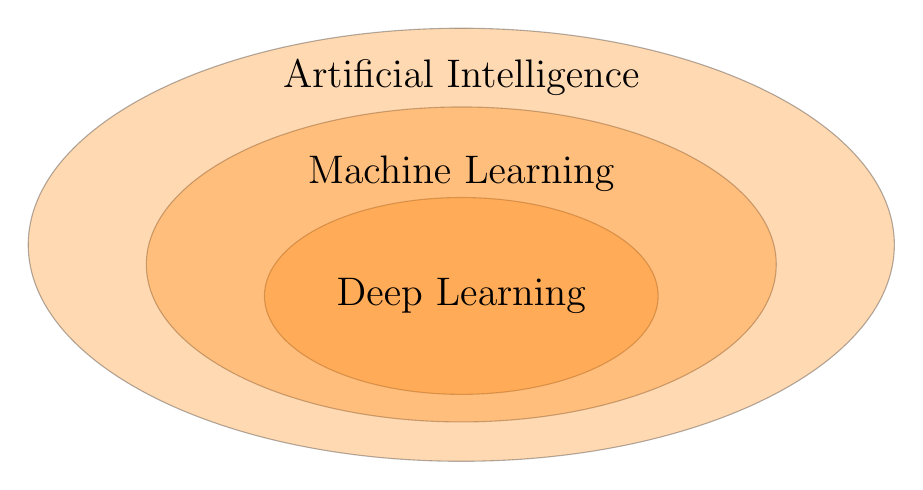
\begin{tikzpicture}
        \draw [black, fill=orange, opacity = 0.3]  (2, -0.65) ellipse (2.5 and 1.25); % DL 
        \draw [black, fill=orange, opacity = 0.3]  (2, -0.25) ellipse (4 and 2); % ML
        \draw [black, fill=orange, opacity = 0.3]  (2, 0) ellipse (5.5 and 2.75);     % AI
        \node at ($(2, 2.125)$) {\Large Artificial Intelligence}; % +(2 and -0.65)
        \node at ($(2, 0.9)$) {\Large Machine Learning};
        \node at ($(2, -0.65)$) {\Large Deep Learning};

    \end{tikzpicture}
    
    \caption{Graph illustrating the subfields of AI. ML is a subfield of AI, DL is again a subfield of ML. The sketch is inspired by Figure 1.1 in \cite{chollet_book}.}
    \label{fig:subcategories_AI}
\end{figure}
%AI dates back to the fifties. Pioneers was debating if it was possible to \textit{automatize task normally performed by humans}. 
Three factors determine advances in the field of AI: data, hardware, and algorithms. \textbf{cite Chollet book} This explains why there often is a significant time gap between the idea and breakthroughs of architectures. Convolutional neural networks (CNNs) being developed in the eighties, lying in hibernation until 2012, when AlexNet (a CNN architecture) wins Image net competition, a image recognition contest. \textbf{cite something} %Long short term memory was invented in 1997. Breakthough in X. 

AI started by automating tasks normally performed by humans. Computer chess is the longest studied problem in the history of artificial intelligence. Therefore the advancements in computer chess provide good examples on the evolution of AI. In 1951, Alan Turing was the first to publish a program, on paper, capable of playing a entire game of chess. Starting with explicitly trained programs. This falls in the category of AI and not ML. \textit{Learning, in the context of ML, describes the automatic search for a better representations.} ML strives to go beyond what we know. This kind of computer chess is fed with many examples of played chess game, frame by frame. Given data and the answers, the goal of ML is to deduct the rules (a program). \textbf{cite something}
The network is presented with many examples and is trained, rather than explicitly programmed. Geoscientists may be more familiar with the phrasing calibrating when it comes to statistical models, which essentially is the same thing. Deep in the context of \textit{deep learning} relates to the number of layers contributing to a network. DL expands the ideas from ML using deeper network, e.g. more layers. A layer is a set of nodes. The connections between the layers are the trained units, also known as weights. After the invention of deep learning, traditional machine learning is sometimes referred to as shallow learning. Linear regression (LR) is ML algorithm predating computers which is still useful today. Traditional LR can be derived using shallow learning methods.
%ML is often referred to as shallow learning since its concerned  \textcolor{kan du droppe "its concerned"? og heller skrive " ML is often referred to as shallow learning since its training structure consist of one or two layers"?} with training structures with one or two layers. 

% Explain glossaries or words that are used a lot.
Intelligence, in the context of artificial intelligence, is still a topic of debate. Traditionally, a machine would be considered intelligent if it would beat a human at a given task. For computer chess, this was achieved in 1997 when IBM's DeepBlue beat Gary Karsparov. Researchers had learned how to build a chess-playing AI. Nothing that could generalize to anything other similar boardgames. In retrospect, it might be possible that this particular architecture would not be informative about human intelligence. See the paper from to get more information about the specifics \textbf{find paper}. Researchers became aware that they had learned less to nothing about how the human mind works. Based phsycology studies its clear that the game of chess involves complex reasoning, search, perceptual and memorial processes. While one can solve chess using these abilities, one can also solve chess by taking radical shortcuts orthogonal to human cognition. This idea about machines are intelligent if they beat humans at a particular task has later been abandoned. \textbf{chollet google artikkel}

There are lot of different types of machine learning, suitable for solving different tasks. Figure \ref{fig:machine_learning_categories} shows the types of ML and their subcategories. In order to keep this section as general as possible, it describes subcategories of machine learning. These subcategories also exist for deep learning, but in order to keep this as general they are described from the above level. Keep in mind that their deep learning cousins can be referred to by simply adding the prefix 'deep'. The frontier of chess playing programs is AlphaZero. The deep reinforcement learning architecture trained is using self-play. Without having any previous knowledge of rules. 
%Supervised learning is the part of machine learning concerned with learning the relation between input data, x and labelled data, y. Regression predict continuous values. Replicating a function. Classification is discrete, since it assigns a category to the input. 
%Reinforcement learning is a goal-oriented algorithms, most known for playing chess, solving labyrinths and lately \textcolor{red}{for?} active flow control \textbf{Cite Jean Rau, three papers}. \textcolor{red}{(Nytt avsnitt?)} 
%Unsupervised learning tries to detect patterns in unlabelled data. This includes clustering and dimensionality reduction. Dimensionality reduction has been used by climatologist for decades in order to remove seasonal variation \textbf{cite Benestad}. Unsupervised and reinforcement learning is out of the scope of this thesis and will not be discussed further.
%author : Hanna Svennevik
\begin{figure}[hp]
    \centering
    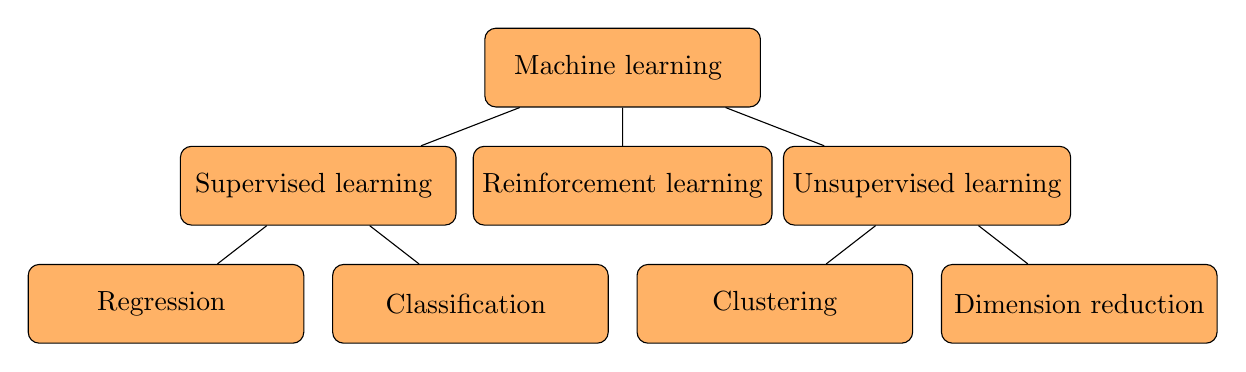
\begin{tikzpicture}[sibling distance=11em,
  every node/.style = {shape=rectangle, rounded corners,
    draw, align=center, 
    %top color=white, bottom color=cyan!20,
    fill=orange!60, minimum width=3.5cm, minimum height = 1.0cm}]]
  \node { Machine learning }
    child { node {  Supervised learning  } 
        child { node {  Regression   } }
        child { node {  Classification  } }
    }
    child {node {Reinforcement  learning}}
    child {node {Unsupervised learning}
           child { node {Clustering}}
           child { node {Dimension reduction}}};
\end{tikzpicture}
    \caption{The graph shows the different type of machine learning and their subcategories.}
    \label{fig:machine_learning_categories}
\end{figure} 

\begin{itemize}
    \item \textbf{Supervised learning}: part of machine learning concerned with learning the relation between input data, x and labelled data, y.
    \begin{itemize}
        \item Regression\\predict continuous values. Replicating a function.
        \item Classification\\discrete, since it assigns a category to the input.
    \end{itemize}
    \item \textbf{Unsupervised learning}: Detecting patterns in unlabeled data.
    \begin{itemize}
        \item Clustering\\Grouping a set of data points into a predescribed number of groups
        \item Dimension reduction\\Reducing the number of random variables under consideration.
    \end{itemize}
    \item \textbf{Reinforcement learning}: Goal oriented algorithms.
\end{itemize}

\subsection{Autoregressive models} \label{sec:ARmodels}
The autoregressive model (AR) is a form of linear model where values from previous time steps are included as predictor variables. 
\begin{equation} \label{eq:AR_traditional}
    \hat{Y}_n = \hat{\beta}_0 + \sum_{i = 1}^{N} Y_{n-i} \hat{\beta}_{i}
\end{equation}
Equation \eqref{eq:AR_traditional} describes how to make a prediction based on the optimal weights, $\beta_i$. Here, $n$ denotes a particular time step, while $N$ denotes the order of the model, also known as number of previous time steps. $\beta_0$ is the bias, and $i$ is a counter going backward in time.
\begin{equation} \label{eq:AR_expression}
    \hat{Y}_n = \hat{\beta}_0 + \sum_{j=1}^p X_j\hat{\beta}_j + \sum_{i = 1}^{N} Y_{n-i}\hat{\beta}_{i}
\end{equation}
Expanding the traditional AR model to include other predictors, $X$ yields the expression in Equation \ref{eq:AR_expression}. $p$ denotes the number of predictors. The other symbols are described above referring to Equation \ref{eq:AR_traditional}.
\begin{equation} \label{eq:AR_solution}
    \hat{ \beta } = \left( \textbf{X}^{*^T}\textbf{X}^* \right)^{-1}\textbf{X}^*\bar{y}
\end{equation}
Let $X^*$ be the concatenation of X and Y. In mathematical terms, $X^*=[X, Y]$. Using mean squared error loss, there exist an analytical solution to the optimization problem. 

The expression for finding the optimal solution, $\beta_0,...\beta_i$, in a matrix form is given in Equation \eqref{eq:AR_solution}. The optimal solution is the best solution based on the training data available. The analytical solution is computationally very fast, as long as the matrix $X^*^TX^*$ is non-singular and thus its inverse exits.

\section{Artificial Neural Networks} \label{sec:artificial neural networks}
\begin{figure}[hp]
\centering
\def\layersep{2.5cm}
\begin{tikzpicture}[shorten >=1pt,->,draw=blue, node distance=\layersep]
    \tikzstyle{every pin edge}=[<-,shorten <=1pt]
    \tikzstyle{neuron}=[circle,fill=black!25,minimum size=17pt,inner sep=0pt]
    \tikzstyle{input neuron}=[neuron, fill=green];
    \tikzstyle{output neuron}=[neuron, fill=red];
    \tikzstyle{hidden neuron}=[neuron, fill=cyan];
    \tikzstyle{annot} = [text width=4em, text centered]

    \node[input neuron] (I-1) at (0,-1) {}; % {$T_{2m}$};
    \node[input neuron] (I-2) at (0,-2) {}; % {$q_v$};
    \node[input neuron] (I-3) at (0,-3) {}; % {$RH$};
    \node[input neuron] (I-4) at (0,-4) {}; % {$p_s$};

    % Draw the input layer nodes
    %\foreach \name / \y in {1,...,4}
    % This is the same as writing \foreach \name / \y in {1/1,2/2,3/3,4/4}
    %    \node[input neuron, pin=left:Input \#\y] (I-\name) at (0,-\y) {};

    % Draw the hidden layer nodes
    \foreach \name / \y in {1,...,5}
        \path[yshift=0.5cm]
            node[hidden neuron] (H-\name) at (\layersep,-\y cm) {};

    % Draw the output layer node
    \node[output neuron, right of=H-2] (O) {};
    \node[output neuron, right of=H-3] (O1) {};
    \node[output neuron, right of=H-4] (O2) {};


    % Connect every node in the input layer with every node in the
    % hidden layer.
    \foreach \source in {1,...,4}
        \foreach \dest in {1,...,5}
            \path (I-\source) edge (H-\dest);

    % Connect every node in the hidden layer with the output layer
    \foreach \source in {1,...,5}
        \path (H-\source) edge (O);
        %\path (H-\source) edge (o1);
        %\path (H-\source) edge (o2);

    % Does the same thing the loop does had to do it manually tho
    \path (H-1) edge (O1);
    \path (H-2) edge (O1);
    \path (H-3) edge (O1);
    \path (H-4) edge (O1);
    \path (H-5) edge (O1);
    
    \path (H-1) edge (O2);
    \path (H-2) edge (O2);
    \path (H-3) edge (O2);
    \path (H-4) edge (O2);
    \path (H-5) edge (O2);

    % Annotate the layers
    \node[annot,above of=H-1, node distance=1cm] (hl) {Hidden layer};
    \node[annot,left of=hl] {Input layer};
    \node[annot,right of=hl] {Output layer};
\end{tikzpicture}

\caption{2-layer neural network. The connections between the layers are the weights. The input layer has four units, the hidden layer has five and the output layer has three. In total there is 35 parameters in this network (37 if bias is included). The sketch is based on the example from Skissen bygger viderer på eksempelet fra \href{http://www.texample.net/tikz/examples/neural-network/}{http://www.texample.net/tikz/examples/neural-network/}}
\label{fig:one_layer_mlp}
\end{figure}
Artificial neural networks (ANN) are composed of artificial neurons and weights. Figure \ref{fig:one_layer_mlp} illustrates nodes as circles and weights as arrows. It is a example of a 2-layer ANN. The nodes are structured in layers, illustrated using different colors. The input layer containing four input nodes, the hidden layer, five nodes and the output layer, three nodes. The dimensions of the input and output layers are determined by the task at hand. The number of hidden layers and the number of nodes are tunable parameters, called hyperparameteres. Neurons of one layer is only connected to the immediately preceding and following layers. Weights are the connections between nodes in neighbouring layers. All networks have input, output and zero or more hidden layers. Large networks of these simple neurons are able to perform complex calculations. 
\begin{figure}[hp!]
\centering
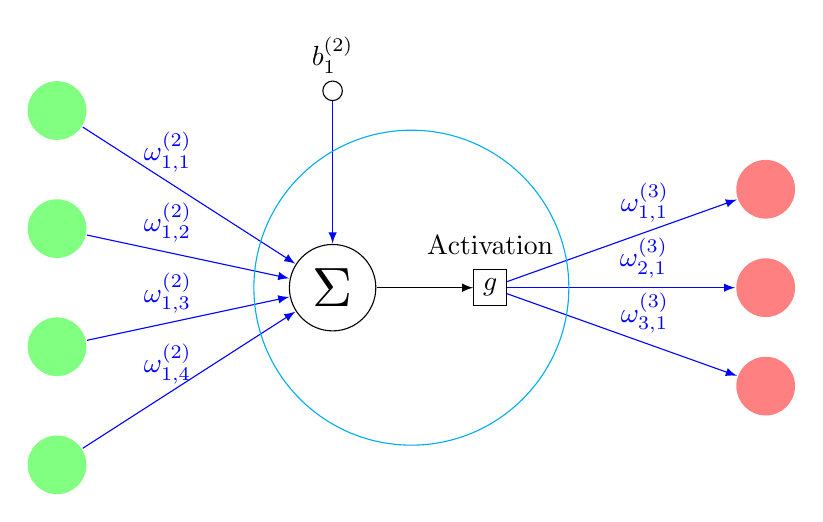
\begin{tikzpicture}[>=latex]
\path
(0,0)     node[circle,draw,scale=2,inner sep=2pt] (S) {$\Sigma$}
+(90:2.5) node[circle,draw,inner sep=2.5pt] (b) {}
          node[above=1mm] {$b_1^{(2)}$}
+(-3.5,2.25)  node[circle,scale=2.25,fill=green!50]  (x1) {} %{$T_{2m}$}
+(-3.5,0.75)  node[circle,scale=2.25,fill=green!50]  (x2) {} %{$q_v$}
+(-3.5,-0.75) node[circle,scale=2.25,fill=green!50]  (x3) {} %{$RH$}
+(-3.5,-2.25) node[circle,scale=2.25,fill=green!50]  (x4) {} %{$p_s$}
(2,0)    node[draw] (g) {$g$} node[above=3mm]{Activation}

+(3.5,1.25)  node[circle,scale=2.25,fill=red!50]  (y1) {}
+(3.5,0)  node[circle,scale=2.25,fill=red!50]  (y3) {}
+(3.5,-1.25) node[circle,scale=2.25,fill=red!50]  (y2) {};

\draw[->, black] (S)--(g);
\draw[->, blue] (b)--(S);
\draw[->, blue] (g)--(y1) node[pos=.6,above, blue]{$\omega_{1,1}^{(3)}$};
\draw[->, blue] (g)--(y2) node[pos=.6,above, blue]{$\omega_{3,1}^{(3)}$};
\draw[->, blue] (g)--(y3) node[pos=.6,above, blue]{$\omega_{2,1}^{(3)}$};

\draw[->, blue] (x1)--(S) node[pos=.4,above, blue]{$\omega_{1,1}^{(2)}$};
\draw[->, blue] (x2)--(S) node[pos=.4,above, blue]{$\omega_{1,2}^{(2)}$};
\draw[->, blue] (x3)--(S) node[pos=.4,above, blue]{$\omega_{1,3}^{(2)}$};
\draw[->, blue] (x4)--(S) node[pos=.4,above, blue]{$\omega_{1,4}^{(2)}$};
\draw[cyan] (1,0) circle(2);
\end{tikzpicture}

\caption{Computational graph showing the components participating in the activation of a neuron in the hidden layer. This example shows a 2-layer neural network with four input nodes and three output nodes. The number of nodes in the hidden layer doesn't affect the activation of the other nodes in the same layer. The sum of the weighted input and bias is passed to the activation function,
inside the hidden layers. Producing the activation of the neuron. This is again passed to the output neurons. Modified skecth based on \href{https://tex.stackexchange.com/questions/505741/architecture-neural-network-with-weights}{https://tex.stackexchange.com/questions/505741/architecture-neural-network-with-weights}. }
\label{fig:activation_one_node}
\end{figure}
Figure \ref{fig:activation_one_node} shows the computation which takes place in a node in the hidden layer, a cyan dot in Figure \ref{fig:one_layer_mlp}. The sum of the weighted input and bias are sent trough the activation function, g. 
\begin{equation} \label{eq:ANN_forward_pass}
    y = g(\sum_{i=1}^n w_{L, i} x_i + b_L)
\end{equation}
The activation in a arbitrary layer, L is given by Equation \eqref{eq:ANN_forward_pass}, where $b_L$ is the bias and $w_L$ is the weights matrix and $n$ is the number of input nodes. The weighted activation is then passed to the output nodes, the red dots. 

\subsection{Convolutional neural networks} \label{sec:convolutional neural network}
Computer vision is a field of artificial intelligence concerned with interpreting the visual world. One popular structure for visual tasks are the convolutional neural network. %Its said to resemble the visual cortex, the centre in the brain which processes the visual information. 
Computer see images as a grid of numbers. Often decoded in red, green and blue (RGB) channels. Each of each of the grid cells, also called pixels, contain the signal from the color decoded into numbers ranging from 0 to 255. The machine needs to learn how to extract the necessary information about these pixels to perform a task. More layers increases the models ability to extract these complex structures. Resulting in an improved model performance. 
% kilde https://tex.stackexchange.com/questions/522118/visualizing-matrix-convolution 
\begin{figure}[hp]
    \centering
    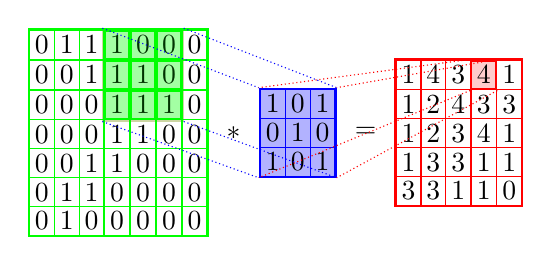
\begin{tikzpicture}[mmat/.style={matrix of math nodes,column sep=-\pgflinewidth/2,
   row sep=-\pgflinewidth/2,cells={nodes={draw,inner sep=2pt,thin}},draw=#1,thick, inner sep=0pt},
   mmat/.default=green,
   node distance=0.3em]
   
 \matrix[mmat](mat1){
         0 & 1 & 1 & |[draw=green,thick,fill=green!20,alias=1]| 1 & |[draw=green,thick,fill=green!20,alias=0]| 0 & |[draw=green,thick,fill=green!20,alias=]| 0 & 0 \\ 
         0 & 0 & 1 & |[draw=green,thick,fill=green!20,alias=1]|1 & |[draw=green,thick,fill=green!20,alias=1]|1 &|[draw=green,thick,fill=green!20,alias=0]| 0 & 0 \\ 
         0 & 0 & 0 & |[draw=green,thick,fill=green!20,alias=1]|1 &|[draw=green,thick,fill=green!20,alias=1]| 1 & |[draw=green,thick,fill=green!20,alias=1]|1 & 0 \\ 
         0 & 0 & 0 & 1 & 1 & 0 & 0 \\ 
         0 & 0 & 1 & 1 & 0 & 0 & 0 \\ 
         0 & 1 & 1 & 0 & 0 & 0 & 0 \\ 
         0 & 1 & 0 & 0 & 0 & 0 & 0 \\ 
         };
 \node[fit=(mat1-1-4)(mat1-3-6),inner sep=0pt, draw, green, thick, fill = green, opacity = 0.2](f1){};        
 
 \node[right=of mat1] (mul) {$*$};      
 \matrix[mmat=blue,fill=blue!30,right=of mul](mat2){    
     1 & 0 & 1 \\ 
     0 & 1 & 0 \\ 
     1 & 0 & 1 \\ };
 \node[right=of mat2] (eq) {$=$};       
 \matrix[mmat,right=of eq, draw = red](mat3){    
     1 & 4 & 3 & |[draw=red,thick,fill=red!20,alias=4]|4 & 1 \\ 
     1 & 2 & 4 & 3 & 3 \\ 
     1 & 2 & 3 & 4 & 1 \\ 
     1 & 3 & 3 & 1 & 1 \\ 
     3 & 3 & 1 & 1 & 0 \\ 
 };
 \foreach \Anchor in {south west,north west,south east,north east}
 {\draw[blue,densely dotted] (f1.\Anchor) -- (mat2.\Anchor); 
 \draw[red,densely dotted] (4.\Anchor) -- (mat2.\Anchor);}
 \begin{scope}[on background layer]
  \fill[red!20] (f1.north west) rectangle (f1.south east);
 \end{scope}
 
 
\end{tikzpicture}
    \caption{Diagram showing a convolutional operation. Inspired by \textbf{Cite}
    \href{https://tex.stackexchange.com/questions/522118/visualizing-matrix-convolution}{https://tex.stackexchange.com/questions/522118/visualizing-matrix-convolution}}
    \label{fig:convolution}
\end{figure}
A convolution is a mathematical operation. The sum over element wise multiplication. This is illustrated in Figure \ref{fig:convolution}. The filter is blue, this is placed over the filled green section, producing the red output pixel. The entire red grid is called a feature map (output map). The blue grid is the input, and as you can see only parts of the image (the filled) blue section contributes to the activation, in this examlpe the value 4. \textit{Receptive field} is known as the pixels contributing to the activation in a pixel (i.e. the value). For instance the receptive field of the filled red pixel is the filled green submatrix.


\begin{figure}
    \centering
    
    \begin{tikzpicture}[scale=2,every node/.style={minimum size=1cm},on grid]
    % slanting: production of a set of n 'laminae' to be piled up.
    % N=number of grids.
    \begin{scope}[
            yshift=-100, xshift= 0, every node/.append style={
            yslant=0.5, xslant=-1.3}, yslant=0.5, xslant=-1.3
            ]
        % opacity to prevent graphical interference
        \draw[red, very thick, fill = white]  (0, 0) rectangle (1.5, 2.1);
        \draw[step=3mm, thin, red] (0, 0) grid (1.5, 2.1);   % defining grids
        \draw[red, very thick] (0, 0) rectangle (1.5, 2.1); % marking borders    
        
        % pixel closest to output layes
        \coordinate (bl) at (0.16, 1.92);
        \node at (bl) [fill=red!80, square, scale=0.65] {};
        
        %last pixel
        \coordinate (pi) at (0.5, 1.92);
        \node at (pi) [fill=red!60, square, scale=0.65] {};
        
        % rightmost pixel
        \coordinate (cy) at (0.16, 0.16);
        \node at (cy) [fill=red!40, square, scale=0.64] {};
        
        \coordinate (input_c) at (0, 2.1);
        %\node at (corner) [fill=yellow, square, scale=0.64] {s};        
        
        \end{scope}
    
        \begin{scope}[
            yshift=-160,every node/.append style={
            yslant=0.5,xslant=-1.3},yslant=0.5,xslant=-1.3
                      ]
            % Marking border
            \draw[blue, very thick, fill = gray!70] (0,0) rectangle (2.1, 2.7);
            \draw[blue, very thick, fill = blue!20] (0.33, 0.33) rectangle (1.8, 2.4);
            \draw[step=3mm, thin, gray] (0,0) grid   (2.1, 2.7);  % defining grid padding
            \draw[step=3mm, thick, blue] (0.33, 0.33) rectangle (1.8, 2.4); % defining grids
            \draw[black, very thick] (0,0) rectangle (2.1, 2.7);% marking borders   
            % \draw[black,very thick, fill = blue!50] (0,0) rectangle (3,3);

            \coordinate (s1) at (0, 2.7);
            %\node at (s1) [fill=blue, circle, scale=0.5] {$s$};
            \coordinate (s2) at (0, 1.8);
            %\node at (s2) [fill=pink, circle, scale=0.5] {$s$};
            \coordinate (s3) at (0.9, 1.8);
            %\node at (s3) [fill=yellow, circle, scale=0.5] {$s$};
            \coordinate (s4) at (0.9, 2.7);
            %\node at (s4) [fill=cyan, circle, scale=0.5] {$s$};
                      
            \draw[draw=green!20, very thick, line join=round, dashed, fill = green!20] %  opacity=.2, 
                  (0,  2.7) -- 
                  (0,  1.8) --
                  (0.9,  1.8) --
                  (0.9,  2.7) -- cycle ;
                
            \draw[fill=white, draw=green!20, opacity=1, very thick, line join=round]
            (s4) -- (bl);
            
            \draw[fill=white, draw=green!20, opacity=1, very thick, line join=round]
            (s3) -- (bl);
 
            \draw[fill=white, draw=green!20, opacity=1, very thick, line join=round]
            (s2) -- (bl);
            
            \draw[fill=white, draw=green!20, opacity=1, very thick, line join=round]
            (s1) -- (bl);
           
           %%%%%%%%%%%%%%%%%%%%%%%% PINK
            \coordinate (s5) at (0.333, 2.7);
            %\node at (s5) [fill=blue, circle, scale=0.5] {$s$};

            \coordinate (s6) at (0.333, 1.8);
            %\node at (s6) [fill=pink, circle, scale=0.5] {$s$};

            \coordinate (s7) at (1.2333, 1.8);
            %\node at (s7) [fill=yellow, circle, scale=0.5] {$s$};

            \coordinate (s8) at (1.2333, 2.7);
            %\node at (s8) [fill=cyan, circle, scale=0.5] {$s$};
           
           
           
            \draw[draw=green!40, very thick, line join=round, opacity=.2, fill = green!40] %  opacity=.2, 
                  (s5) -- (s6) -- (s7) -- (s8) -- cycle;

            \draw[fill=white, draw=green!40, opacity=1, very thick, line join=round, dashed]
            (s5) -- (pi);
            
            \draw[fill=white, draw=green!40, opacity=1, very thick, line join=round, dashed]
            (s6) -- (pi);
 
            \draw[fill=white, draw=green!40, opacity=1, very thick, line join=round, dashed]
            (s7) -- (pi);
            
            \draw[fill=white, draw=green!40, opacity=1, very thick, line join=round, dashed]
            (s8) -- (pi);
            
            %%%%%%%%%%%%%%%%%%%%%%%% CYAN
            \coordinate (s9) at (0, 0);
            %\node at (s5) [fill=blue, circle, scale=0.5] {$s$};

            \coordinate (input_layer) at (0.32, 0.32);
            %\node at (input_layer) [fill=blue, circle, scale=0.5] {$s$};

            \coordinate (s10) at (0, 0.9);
            %\node at (s6) [fill=pink, circle, scale=0.5] {$s$};

            \coordinate (s11) at (0.9, 0.9);
            %\node at (s7) [fill=yellow, circle, scale=0.5] {$s$};

            \coordinate (s12) at (0.9, 0);
            %\node at (s8) [fill=cyan, circle, scale=0.5] {$s$};
           
            % Adding coordinates for padding
            \coordinate (p1) at (2.1, 0);
            \coordinate (p2) at (1.8, 0);

            \draw[draw=green!60, very thick, line join=round, dashed, opacity=.6, fill = green!60] %  opacity=.2, 
                  (s9) -- (s10) -- (s11) -- (s12) -- cycle;

            \draw[fill=white, draw=green!60, opacity=.6, very thick, line join=round]
            (s9) -- (cy);
            
            \draw[fill=white, draw=green!60, opacity=.6, very thick, line join=round]
            (s10) -- (cy);
 
            \draw[fill=white, draw=green!60, opacity=.6, very thick, line join=round]
            (s11) -- (cy);
            
            \draw[fill=white, draw=green!60, opacity=.6, very thick, line join=round]
            (s12) -- (cy);
            
        \end{scope} %end of drawing grids
    
       \draw[-latex,thick](-1, -6)node[left, scale=1.3]{Input layer}
             to[out=0, in=90] (input_layer);  	
            
        \draw[-latex,thick](2.7, -4.25)node[above, scale=1.3]{Zero padding}
             to[out=0, in=90] (p1);  
        \draw[-latex,thick](2.7, -4.25)node[above, scale=1.3]{}
             to[out=0, in=90] (p2);      
             
       \draw[-latex,thick](-3, -2.5)node[left, scale=1.3]{Output layer}
             to[out=0,in=90] (input_c);  	
        
        \draw[-latex,thick](-4, -5)node[left, scale=1.3]{$f_w = 3$}
               to[out=0,in=90] (s1);  	
        \draw[-latex,thick](-4, -5)node[left]{}
              to[out=0,in=90] (s2);  	
            
        \draw[-latex,thick](-3.7, -4.4)node[left, scale=1.3]{$f_h = 3$}
               to[out=0,in=90] (s1);  	
        \draw[-latex,thick](-3.7, -4.4)node[left]{}
              to[out=0,in=90] (s4);  
              
    \end{tikzpicture}
    
    \caption{The illustration shows the connections between 
    input and output layer. This example uses a $3\times 3$-filter (green), zero-padding (gray) resulting in equal dimensions for input (blue) and output (red). The different colors illustrate the connections between input and output pixels. The input pixels contributing to the output, is called the receptive field. The zero padding is added to keep the input shape. Its is inspired by 13-3 in O'Reiley (page 362).  }
    \label{fig:convolution_padding}
\end{figure}
Convolving a filter over the input image generates a feature map. If it happens to be the last layer, it is common to refer to the results as the output instead. Even though there is no difference. Figure \ref{fig:convolution_padding} shows a 2D-convolution with filter of size $3\times 3$. Filters are often square (not a strict requirement) and the height, $f_h$ and $f_w$ are odd numbers (not a strict requirement either). The origin is the position of the kernel which is above the current output pixels. The connections between the layers are intended to illustrate the part contributing to the pixel, as well as highlighting the receptive field. With the purpose of including the signal from the boundary and or preserving the input shape. The gray shaded area is the padded with zeros. 
\begin{figure}
    \centering
   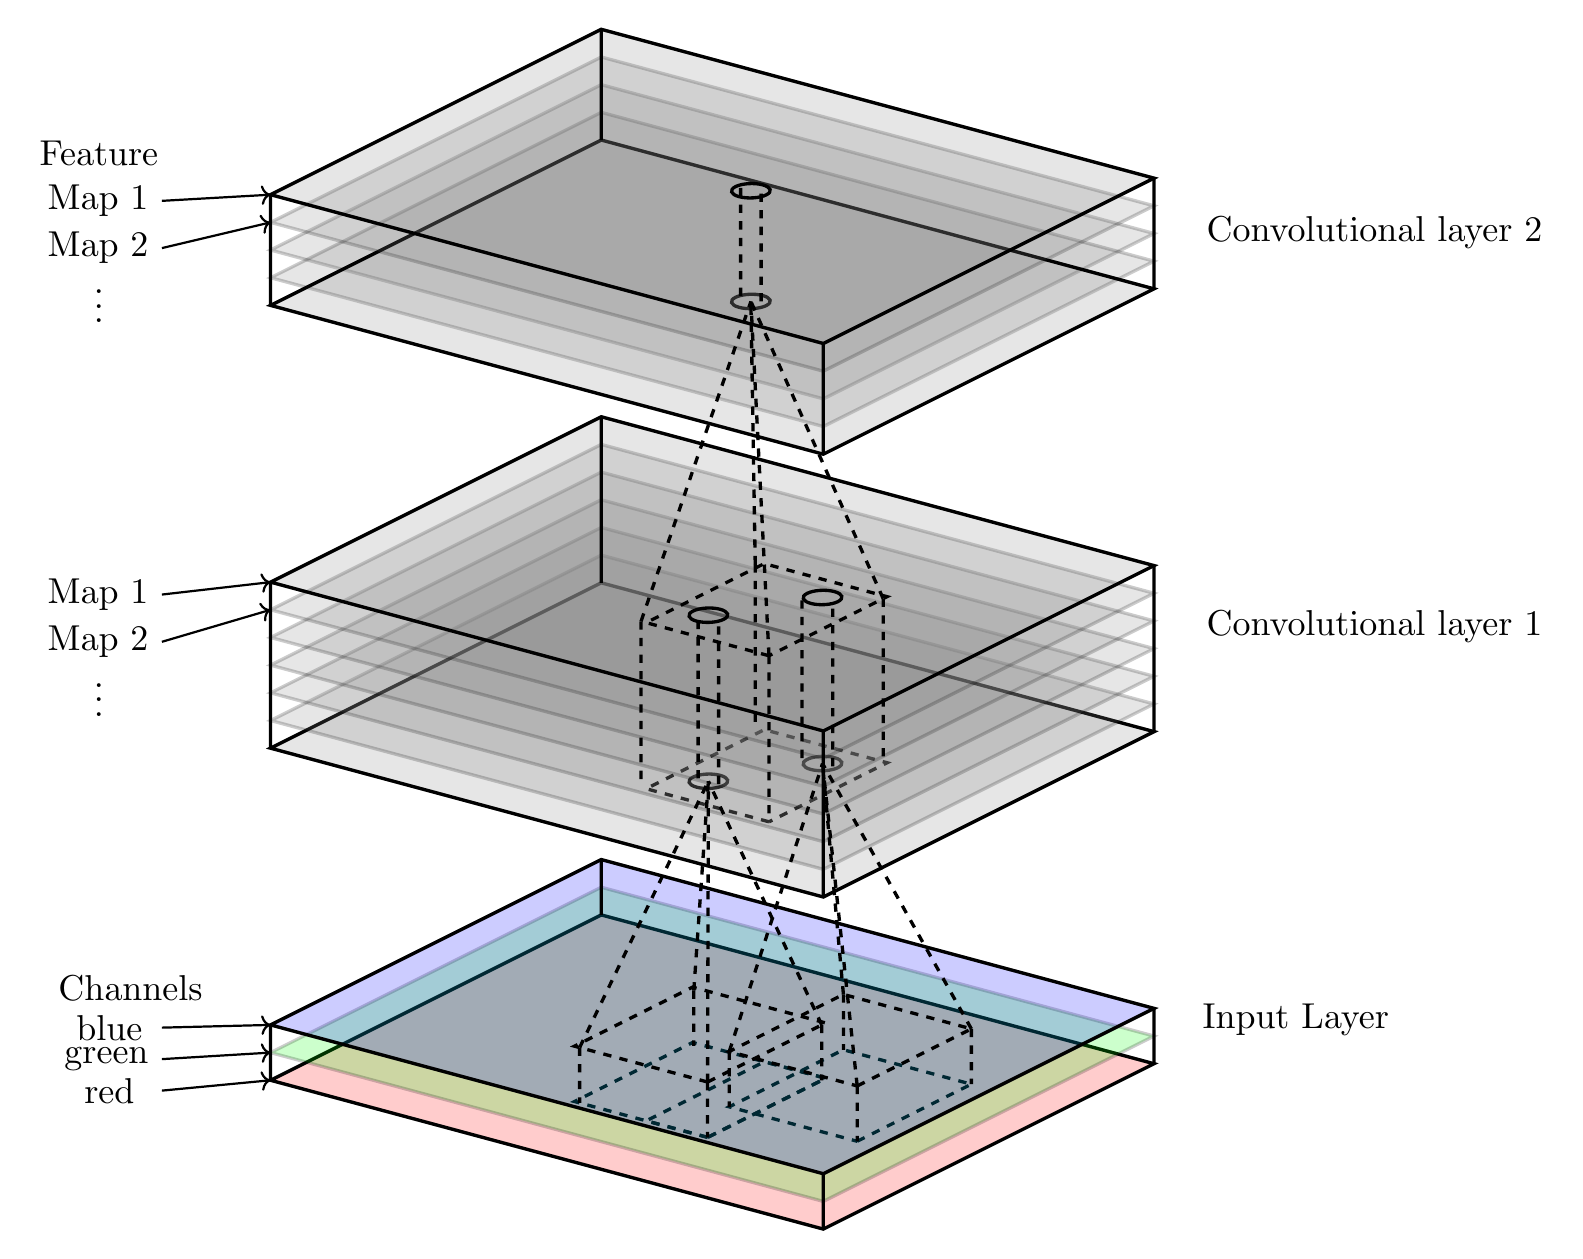
\begin{tikzpicture}[scale=2,every node/.style={minimum size=1cm},on grid]
    % slanting: production of a set of n 'laminae' to be piled up.
    % N=number of grids.

        \begin{scope}[
            yshift=-200,every node/.append style={
            yslant=0.5,xslant=-1.3},yslant=0.5,xslant=-1.3
                      ]
            \draw[black, very thick, fill = red, opacity = 0.2] (0,0) rectangle (2.1, 2.7); % marking borders 
            \draw[black, very thick] (0,0) rectangle (2.1, 2.7); % marking borders 

            \coordinate (s9) at (0, 0);
            %\node at (s9) [fill=blue, circle, scale=0.5] {$s$};
            \coordinate (s10) at (0, 2.7);
            %\node at (s10) [fill=pink, circle, scale=0.5] {$s$};
            \coordinate (s11) at (2.1, 0);
            %\node at (s11) [fill=yellow, circle, scale=0.5] {$s$};
            \coordinate (s12) at (2.1, 2.7);
            %\node at (s12) [fill=cyan, circle, scale=0.5] {$s$};
            \coordinate (h_re) at (0, 2.7);
            %\node at (h_re) [fill=red, circle, scale=0.5] {$s$};
                                   
            % begynner i punkt (x, y) rectangle (x dim, y dim)
            \draw[black, very thick, dashed] (0.5, 0.95) rectangle (1.25, 1.25);
            \coordinate (o1) at (0.5, 0.95);
            %\node at (p1) [draw=black, very thick, circle, scale=0.3] {};
            \coordinate (o2) at (0.5, 0.95+1.25/2);
            %\node at (p2) [draw=black, very thick, circle, scale=0.3] {};
            \coordinate (o3) at (0.5+1.25/2+0.1, 0.95);
            %\node at (p3) [draw=black, very thick, circle, scale=0.3] {};
            \coordinate (o4) at (0.5+1.25/2+0.1, 0.95+1.25/2);
            %\node at (p4) [draw=black, very thick, circle, scale=0.3] {};

           
            % begynner i punkt (x, y) rectangle (x dim, y dim)
            \draw[black, very thick, dashed] (0.5, 0.95) rectangle (1.25, 1.6);
            \coordinate (z1) at (0.5, 0.95);
            %\node at (q1) [draw=black, very thick, circle, scale=0.3] {};
            \coordinate (z2) at (0.5, 0.95+1.25/2);
            %\node at (q2) [draw=black, very thick, circle, scale=0.3] {};
            \coordinate (z3) at (0.5+1.25/2+0.1, 0.95);
            %\node at (q3) [draw=black, very thick, circle, scale=0.3] {};
            \coordinate (z4) at (0.5+1.25/2+0.1, 0.95+1.25/2);
            %\node at (q4) [draw=black, very thick, circle, scale=0.3] {};


            %\draw[black, very thick, dashed] (0.8, 0.45) rectangle (1.25, 1.6);
            \coordinate (x1) at (0.8, 0.45);
            %\node at (u1) [draw=black, very thick, circle, scale=0.3] {};
            \coordinate (x2) at (0.8, 0.45+1.25/2);
            %\node at (u2) [draw=black, very thick, circle, scale=0.3] {};
            \coordinate (x3) at (0.8+1.25/2+0.1, 0.45);
            %\node at (u3) [draw=black, very thick, circle, scale=0.3] {};
            \coordinate (x4) at (0.8+1.25/2+0.1, 0.45+1.25/2);
            %\node at (u4) [draw=black, very thick, circle, scale=0.3] {};
            \draw[black,very thick, dashed]   (x1) -- (x3) -- (x4) -- (x2) --(x1);
        \end{scope} 

        \begin{scope}[
            yshift=-195,every node/.append style={
            yslant=0.5,xslant=-1.3},yslant=0.5,xslant=-1.3
                      ]
            \draw[black, very thick, fill = green, opacity = 0.2] (0,0) rectangle (2.1, 2.7); % marking borders 
            \coordinate (h_input) at (2.1, 0);
            \coordinate (h_bl) at (0, 2.7);
            %\node at (h_bl) [fill=blue, circle, scale=0.5] {$s$};
        \end{scope} 
           
           \draw[thick](3, -5.7)node[scale=1.3]{Input Layer};
           \draw[thick](3.5, -3.2)node[scale=1.3]{Convolutional layer 1};
           \draw[thick](3.5, -0.7)node[scale=1.3]{Convolutional layer 2};
           \draw[thick](-4.6, -0.2)node[scale=1.3]{Feature};
           \draw[thick](-4.6, -1.1)node[scale=1.3]{$\vdots$};
           \draw[thick](-4.6, -3.6)node[scale=1.3]{$\vdots$};
           \draw[thick](-4.4, -5.5)node[scale=1.3]{Channels};
           
        \begin{scope}[
            yshift=-190,every node/.append style={
            yslant=0.5,xslant=-1.3},yslant=0.5,xslant=-1.3
                      ]
            \draw[black, very thick, fill = blue, opacity = 0.2] (0,0) rectangle (2.1, 2.7); % marking borders 
            \draw[black, very thick] (0,0) rectangle (2.1, 2.7); % marking borders 

            \coordinate (s1) at (0, 0);
            \coordinate (s2) at (0, 2.7);
            \coordinate (s3) at (2.1, 0);
            \coordinate (s4) at (2.1, 2.7);

            \draw[black,very thick]   (s9) -- (s1);
            \draw[black,very thick]   (s10) -- (s2);
            \draw[black,very thick]   (s11) -- (s3);
            \draw[black,very thick]   (s12) -- (s4);
                        
            \coordinate (h_gr) at (0, 2.7);

            % begynner i punkt (x, y) rectangle (x dim, y dim)
            \draw[black, very thick, dashed] (0.5, 0.95) rectangle (1.25, 1.6);
            \coordinate (q1) at (0.5, 0.95);
            %\node at (q1) [draw=black, very thick, circle, scale=0.3] {};
            \coordinate (q2) at (0.5, 0.95+1.25/2);
            %\node at (q2) [draw=black, very thick, circle, scale=0.3] {};
            \coordinate (q3) at (0.5+1.25/2+0.1, 0.95);
            %\node at (q3) [draw=black, very thick, circle, scale=0.3] {};
            \coordinate (q4) at (0.5+1.25/2+0.1, 0.95+1.25/2);
            %\node at (q4) [draw=black, very thick, circle, scale=0.3] {};

            %\draw[black, very thick, dashed] (0.8, 0.45) rectangle (1.25, 1.6);
            \coordinate (u1) at (0.8, 0.45);
            %\node at (u1) [draw=black, very thick, circle, scale=0.3] {};
            \coordinate (u2) at (0.8, 0.45+1.25/2);
            %\node at (u2) [draw=black, very thick, circle, scale=0.3] {};
            \coordinate (u3) at (0.8+1.25/2+0.1, 0.45);
            %\node at (u3) [draw=black, very thick, circle, scale=0.3] {};
            \coordinate (u4) at (0.8+1.25/2+0.1, 0.45+1.25/2);
            %\node at (u4) [draw=black, very thick, circle, scale=0.3] {};

            \draw[black,very thick, dashed]   (u1) -- (u3) -- (u4) -- (u2) --(u1);

            % Draws horizontal lines completing the litle cube.
            \draw[black,very thick, dashed]   (q1) -- (z1);
            \draw[black,very thick, dashed]   (q2) -- (z2);
            \draw[black,very thick, dashed]   (q3) -- (z3);
            \draw[black,very thick, dashed]   (q4) -- (z4);
            
            % Draws horizontal lines completing the litle cube.
            \draw[black,very thick, dashed]   (u1) -- (x1);
            \draw[black,very thick, dashed]   (u2) -- (x2);
            \draw[black,very thick, dashed]   (u3) -- (x3);
            \draw[black,very thick, dashed]   (u4) -- (x4);
            
        \end{scope} 

        \draw[black, thick, ->](-4.2, -5.95)node[left, scale=1.3]{green} to (h_bl);
        \draw[thick, ->](-4.2, -6.15)node[left, scale=1.3]{red} to (h_re);
        \draw[thick, ->](-4.2, -5.75)node[left, scale=1.3]{blue} to (h_gr);
        %%%%%%%%%%%%%%%%%%%%%%%% END OF INPUT LAYER 


        \begin{scope}[
            yshift=-140, every node/.append style={
            yslant=0.5,xslant=-1.3},yslant=0.5,xslant=-1.3]
            \draw[black, very thick, fill = gray, opacity = 0.2] (0,0) rectangle (2.1, 2.7); % marking borders 
            % Draws the boundary boxes
            \draw[black, very thick] (0,0) rectangle (2.1, 2.7);
            \coordinate (e5) at (0, 0);
            \coordinate (e6) at (0, 2.7);
            \coordinate (e7) at (2.1, 0);
            \coordinate (e8) at (2.1, 2.7);


            % draw left cylinder
            \coordinate (f) at (0.7, 1.1);
            \node at (f) [draw=black, very thick, circle, scale=0.3] {};
            \coordinate (f1) at (0.7, 1.15);
            %\node at (f1) [draw=red, very thick, circle, scale=0.3] {};
            \coordinate (f2) at (0.7, 1.05);
            %\node at (f2) [draw=red, very thick, circle, scale=0.3] {};
            
            % Draws the other
            \coordinate (g) at (1.1, 0.85);
            \node at (g) [draw=black, very thick, circle, scale=0.3] {};
            \coordinate (g1) at (1.1, 0.95);
            \coordinate (g2) at (1.1, 0.8);
            
            % Drawing the smaller lower 
            \draw[black, very thick, dashed] (0.5, 0.65) rectangle (1.25, 1.25);
            \coordinate (o1) at (0.5, 0.65);
            %\node at (o1) [draw=black, very thick, circle, scale=0.3] {};
            \coordinate (o2) at (0.5, 0.65+1.25/2);
            %\node at (o2) [draw=black, very thick, circle, scale=0.3] {};
            \coordinate (o3) at (0.5+1.25/2+0.1, 0.65);
            %\node at (o3) [draw=black, very thick, circle, scale=0.3] {};
            \coordinate (o4) at (0.5+1.25/2+0.1, 0.65+1.25/2);
            %\node at (o4) [draw=black, very thick, circle, scale=0.3] {};
  
        \end{scope} 
        
        \begin{scope}[
            yshift=-135,every node/.append style={
            yslant=0.5,xslant=-1.3},yslant=0.5,xslant=-1.3
                      ]
            \draw[black, very thick, fill = gray, opacity = 0.2] (0,0) rectangle (2.1, 2.7); % marking borders 
        \end{scope} 
    
        \begin{scope}[
            yshift=-130,every node/.append style={
            yslant=0.5,xslant=-1.3},yslant=0.5,xslant=-1.3
                      ]
            \draw[black, very thick, fill = gray, opacity = 0.2] (0,0) rectangle (2.1, 2.7); % marking borders 
        \end{scope} 
    

        \begin{scope}[
            yshift=-125, every node/.append style={
            yslant=0.5,xslant=-1.3},yslant=0.5,xslant=-1.3
                      ]
            \draw[black, very thick, fill = gray, opacity = 0.2] (0,0) rectangle (2.1, 2.7); % marking borders 
            \coordinate (h) at (2.1, 0);
            %\node at (h) [fill=blue, circle, scale=0.5] {$s$};
        \end{scope} 
        
        \begin{scope}[
            yshift=-120,every node/.append style={
            yslant=0.5,xslant=-1.3},yslant=0.5,xslant=-1.3
                      ]
            \draw[black, very thick, fill = gray, opacity = 0.2] (0,0) rectangle (2.1, 2.7); % marking borders 
        \end{scope} 
    
        \begin{scope}[
            yshift=-115,every node/.append style={
            yslant=0.5,xslant=-1.3},yslant=0.5,xslant=-1.3
                      ]
            \draw[black, very thick, fill = gray, opacity = 0.2] (0,0) rectangle (2.1, 2.7); % marking borders 
            
            % Connections to maps
            \coordinate (sec_map_L2) at (0, 2.7);
            %\node at (sec_map_L2) [fill=blue, circle, scale=0.5] {$s$};
            
        \end{scope} 
    
        \begin{scope}[
            yshift=-110,every node/.append style={
            yslant=0.5,xslant=-1.3},yslant=0.5,xslant=-1.3
                      ]
            \draw[black, very thick, fill = gray, opacity = 0.2] (0,0) rectangle (2.1, 2.7); % marking borders 
                    
            % Connections to maps
            \coordinate (sec_map_L1) at (0, 2.7);
            %\node at (sec_map_L1) [fill=blue, circle, scale=0.5] {$s$};
            
          \coordinate (e1) at (0, 0);
          \coordinate (e2) at (0, 2.7);
          \coordinate (e3) at (2.1, 0);
          \coordinate (e4) at (2.1, 2.7);

            \draw[black, very thick] (0,0) rectangle (2.1, 2.7); % draw boundaries
            % draws horizontal lines
            \draw[black,very thick]   (e5) -- (e1);
            \draw[black,very thick]   (e6) -- (e2);
            \draw[black,very thick]   (e7) -- (e3);
            \draw[black,very thick]   (e8) -- (e4);
            
            % begynner i punkt (x, y) rectangle (x dim, y dim)
            \draw[black, very thick, dashed] (0.5, 0.65) rectangle (1.25, 1.25);
            \coordinate (p1) at (0.5, 0.65);
            %\node at (p1) [draw=black, very thick, circle, scale=0.3] {};
            \coordinate (p2) at (0.5, 0.65+1.25/2);
            %\node at (p2) [draw=black, very thick, circle, scale=0.3] {};
            \coordinate (p3) at (0.5+1.25/2+0.1, 0.65);
            %\node at (p3) [draw=black, very thick, circle, scale=0.3] {};
            \coordinate (p4) at (0.5+1.25/2+0.1, 0.65+1.25/2);
            %\node at (p4) [draw=black, very thick, circle, scale=0.3] {};

            % Draws horizontal lines completing the litle cube.
            \draw[black,very thick, dashed]   (p1) -- (o1);
            \draw[black,very thick, dashed]   (p2) -- (o2);
            \draw[black,very thick, dashed]   (p3) -- (o3);
            \draw[black,very thick, dashed]   (p4) -- (o4);
            
            % draw one cylinder
            \coordinate (w) at (0.7, 1.1);
            \node at (w) [draw=black, very thick, circle, scale=0.3] {};
            \coordinate (w1) at (0.7, 1.15);
            %\node at (f1) [draw=red, very thick, circle, scale=0.3] {};
            \coordinate (w2) at (0.7, 1.05);
            %\node at (f2) [draw=red, very thick, circle, scale=0.3] {};
            
            % Draws the other
            \coordinate (r) at (1.1, 0.85);
            \node at (r) [draw=black, very thick, circle, scale=0.3] {};
            \coordinate (r1) at (1.1, 0.95);
            \coordinate (r2) at (1.1, 0.8);

            \draw[black, very thick, dashed]   (f1) -- (w1);
            \draw[black, very thick, dashed]   (f2) -- (w2);

            \draw[black, very thick, dashed]   (g1) -- (r1);
            \draw[black, very thick, dashed]   (g2) -- (r2);


            % Connnection between layers 
            \draw[black,very thick, dashed]   (q1) -- (f);
            \draw[black,very thick, dashed]   (q2) -- (f);
            \draw[black,very thick, dashed]   (q3) -- (f);
            \draw[black,very thick, dashed]   (q4) -- (f);
            
            % Connnection between layers 
            \draw[black,very thick, dashed]   (u1) -- (g);
            \draw[black,very thick, dashed]   (u2) -- (g);
            \draw[black,very thick, dashed]   (u3) -- (g);
            \draw[black,very thick, dashed]   (u4) -- (g);
            

        \end{scope} 
    
    
    
    
    
    %%%%%%%%%%%%%%%%%%%%%%%%%%%%% CONVOLUTIONAL LAYER 2
        
        \begin{scope}[
            yshift=-50,every node/.append style={
            yslant=0.5,xslant=-1.3},yslant=0.5,xslant=-1.3
                      ]
            \draw[black, very thick, fill = gray, opacity = 0.2] (0,0) rectangle (2.1, 2.7); % drawing layer 
            \coordinate (h) at (2.1, 0);
            %\node at (h) [fill=blue, circle, scale=0.5] {$s$};
            
        \end{scope} 

        \begin{scope}[
            yshift=-55,every node/.append style={
            yslant=0.5,xslant=-1.3},yslant=0.5,xslant=-1.3
                      ]
            \draw[black, very thick, fill = gray, opacity = 0.2] (0,0) rectangle (2.1, 2.7); % marking borders 
        \end{scope} 
        
        \begin{scope}[
            yshift=-60,every node/.append style={
            yslant=0.5,xslant=-1.3},yslant=0.5,xslant=-1.3
                      ]
                      
            % The outer box
            \draw[black, very thick, fill = gray, opacity = 0.2] (0,0) rectangle (2.1, 2.7); % marking borders 
            \coordinate (a5) at (0, 0);
            \coordinate (a6) at (0, 2.7);
            \coordinate (a7) at (2.1, 0);
            \coordinate (a8) at (2.1, 2.7);
            \draw[black, very thick] (0,0) rectangle (2.1, 2.7); % draw boundaries
                    
            % The inner box
            \coordinate (h) at (1.1, 1.2); % this should be connected to the next layer
            \node at (h) [draw=black, very thick, circle, scale=0.3] {};
            \coordinate (h1) at (1.1, 1.25);
            \coordinate (h2) at (1.1, 1.15);
            
        \end{scope} 
    
            \begin{scope}[
            yshift=-45,every node/.append style={
            yslant=0.5,xslant=-1.3},yslant=0.5,xslant=-1.3
                      ]
            \draw[black, very thick, fill = gray, opacity = 0.2] (0,0) rectangle (2.1, 2.7); % marking borders 
            
            \coordinate (sec_map) at (0, 2.7);
            %\node at (sec_map) [fill=blue, circle, scale=0.5] {$s$};
            
        \end{scope} 
        
        \begin{scope}[
            yshift=-40,every node/.append style={
            yslant=0.5,xslant=-1.3},yslant=0.5,xslant=-1.3
                      ]
            \draw[black, very thick, fill = gray, opacity = 0.2] (0,0) rectangle (2.1, 2.7); % marking borders 
            \coordinate (a1) at (0, 0);
            \coordinate (a2) at (0, 2.7);
            \coordinate (a3) at (2.1, 0);
            \coordinate (a4) at (2.1, 2.7);

            \draw[black, very thick] (0,0) rectangle (2.1, 2.7); % draw boundaries
            % draws horizontal lines
            \draw[black,very thick]   (a5) -- (a1);
            \draw[black,very thick]   (a6) -- (a2);
            \draw[black,very thick]   (a7) -- (a3);
            \draw[black,very thick]   (a8) -- (a4);
            
            % Draws the cylinder
            \coordinate (i) at (1.1, 1.2);
            \node at (i) [draw=black, very thick, circle, scale=0.3] {};
            \coordinate (i1) at (1.1, 1.25); % for lines
            \coordinate (i2) at (1.1, 1.15); % for lines
            
            % drawing lines
            \draw[black,very thick, dashed]   (i1) -- (h1);
            \draw[black,very thick, dashed]   (i2) -- (h2);

            % Draw the lines connecting the first and second layer.
            \draw[black,very thick, dashed]   (p1) -- (h);
            \draw[black,very thick, dashed]   (p2) -- (h);
            \draw[black,very thick, dashed]   (p3) -- (h);
            \draw[black,very thick, dashed]   (p4) -- (h);

            \coordinate (first_map) at (0, 2.7);
            %\node at (first_map) [fill=blue, circle, scale=0.5] {$s$};

        \end{scope} 
    
        \draw[thick, ->](-4.2, -0.5)node[left, scale=1.3]{Map 1} to (first_map);
        \draw[thick, ->](-4.2, -0.8)node[left, scale=1.3]{Map 2} to (sec_map);
     
        \draw[thick, ->](-4.2, -3)node[left, scale=1.3]{Map 1} to (sec_map_L1);
        \draw[thick, ->](-4.2, -3.3)node[left, scale=1.3]{Map 2} to (sec_map_L2);
     
     
    
    % signed distance
    \end{tikzpicture}    \caption{ Each convolutional layer contains multiple filters, thus producing stack of feature maps. The trailing layer get this stack as input, producing activations based on all channels. For each layer it contains representations of the structures found in the previous layer. The filters are the weights trained to find useful structures. In each convolutional layer multiple of these filters are passed over the image.
    Receptive fields. \textbf{Skal legge til mer, gjør det etter teksten er ok.}}
    \label{fig:conv_layers}
\end{figure} 
 
It is worth noting that the same structures are given different names, based on their position in the network. The output is the feature map resulting from convolving the last layer. Their are both activations, produced based on the input from the previous layer. The number of channels in the first layers and the numbers of feature map in the next layers, both are simply stacks of grids containing values.
\begin{figure}
    \centering
    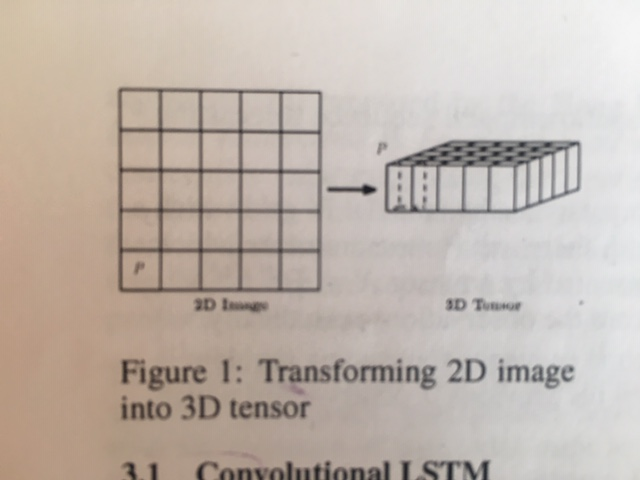
\includegraphics[scale = 0.4]{image_2_3D_tensor.JPG}
    \caption{I consider making this image, to show how a RGB image get turned into channels. Precipitation Nowcastinig paper.}
    \label{fig:RGB_image}
\end{figure}
Working with RGB-images requires 3D-convolution. As mentioned earlier, neural networks are a stack of layers. Each layer is again a stack of channels of feature maps. The output from the previous layer becomes the input to the next layer. To be clear, feature maps, activations and outputs are the same thing. It is the result of convolving the input. The activations are computed based on a input volume, including information across channels. Meaning it knows about all the colors of a RGB-image. Figure \ref{fig:conv_layers} shows a two layer convolutional neural network trained on RGB-images. The input layer is a RGB-image. The first convolutional layer has seven channels (feature maps), these are produced by seven filters. Filters are trained to extract useful features. The second convolutional layer is produced by five filters, all convolving layer 1. It worth noting it is this shallow for illustrative purposes. Networks are usually a lot deeper. Given raw input (i.e. normalized images), the first layers detects low level features like edges, corners and circles. The last layers assemble the features to more complex structures like houses or dogs. The dashed volumes represent the receptive field for different pixels, illustrated as circles. Since each of the layers depend on the previous one, the receptive field of the output node \textbf{give it a name} depends on a large portion of the input image. Small filters allow you to focus on small features in the data. Larger filters allows you to find coarser relations. 

Unlike fully connected layers (see Figure \ref{fig:one_layer_mlp}), the nodes in the output layer are not connected to all the input nodes, only the nodes within their receptive fields. The filters are square, and contains the parameters learned using convolution. This allows you to look for the same structure all of the image. %Reduces the number of trainable parameters and making it more robust against overfitting.

\subsection{Recurrent Nets} \label{sec:reccurent_nets}
% Recurrent betyr tilbakevendende
% Sequential modelling has had a great success in applications such as machine translation and speech recognition 


\begin{figure}[hp]
    \centering
        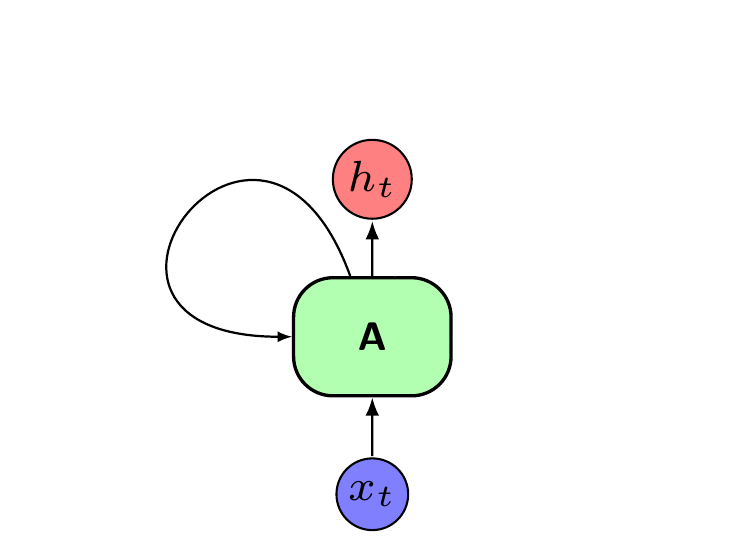
\begin{tikzpicture}[
    % GLOBAL CFG
    font=\sf \scriptsize,
    >=LaTeX,
    % Styles
    cell/.style={% For the main box
        rectangle, 
        rounded corners=5mm, 
        draw,
        very thick,
        },
    operator/.style={%For operators like +  and  x
        circle,
        draw,
        inner sep=-0.5pt,
        minimum height =.01cm,
        },
    function/.style={%For functions
        ellipse,
        draw,
        inner sep=1pt
        },
    ct/.style={% For external inputs and outputs
        circle,
        draw,
        line width = .75pt,
        minimum width=0.2cm,
        inner sep=1pt,
        },
    gt/.style={% For internal inputs
        rectangle,
        draw,
        minimum width=4mm,
        minimum height=3mm,
        inner sep=1pt
        },
    mylabel/.style={% something new that I have learned
        font=\scriptsize\sffamily
        },
    ArrowC1/.style={% Arrows with rounded corners
        rounded corners=.25cm,
        thick,
        },
    ArrowC2/.style={% Arrows with big rounded corners
        rounded corners=.5cm,
        thick,
        },
    ]

%Start drawing the thing...    
    % Draw the cell: 
    \node [cell, minimum height =1.5cm, minimum width=2cm, fill = green!30] (first) at (0,0){\Large \textbf{A}}; % , fill=green

    %\node[ct, label={[mylabel]Cell state}] (c) at (-4,1.5) {\empt{c}{t-1}};
    \node[ct, fill = red!50, scale = 2.25] (h) at (0, 2) {$h_{t}$}; % , fill=blue
    \node[ct, fill = blue!50, scale = 2.25] (x) at (0, -2) { $x_t$}; %, fill = magenta
    \draw [->, ArrowC1] (x) -- (first);
    \draw [->, ArrowC1] (first) -- (h);

    %\node [operator, fill = black, opacity = 1] (a) at (0, 1) { };
    %\node [operator, fill = black, opacity = 1] (d) at (-2, 1) { };
    %\node [operator, fill = black, opacity = 1] (c) at (2, 0) { }; 
    %\node [operator, fill = black, opacity = 1] (b) at (-2, .0) { };

    %\draw [->, ArrowC1] (first) -- (a) -- (d) -- (b)  -- (first);
     
    \draw[-latex, thick] (first) to[out=110,in=180, loop] node[auto] {} (first);  
    \draw[-latex, thick, white] (first) to[out=70,in=360, loop] node[auto] {} (first);  

    %\draw [->] (first) to[loop above] node[auto] {} (first);
    \end{tikzpicture}
    
    \caption{Simple one layer recurrent network. $x_t$ denotes the input, $h_t$ denotes the output/ hidden state of the neuron and A denotes a artificial recurrent unit. Note the output can be different from the hidden state, but it doesn't necessarily have to be. Inspired by \href{http://colah.github.io/posts/2015-08-Understanding-LSTMs/}{http://colah.github.io/posts/2015-08-Understanding-LSTMs/}.}
    \label{fig:rnn}
\end{figure}
Recurrent neural network (RNN) is a class of artificial neural networks. Developed for studying patterns in sequential data such as time series, audio or text. Figure \ref{fig:rnn} shows the structure of a simple RNN. In very simplified terms RNN receives a input, produces an output and passes it back to itself. In Figure \ref{fig:rnn}, A denotes a recurrent unit, $x_t$ denotes the input data and  $h_t$ denotes the hidden state. The output from an arbitrary node, $i$ is $h_i$. The loop explains the origin of the name recurrent neural network. The output at each time step is dependant on the previous inputs.


\begin{figure}[hp]
    \centering
        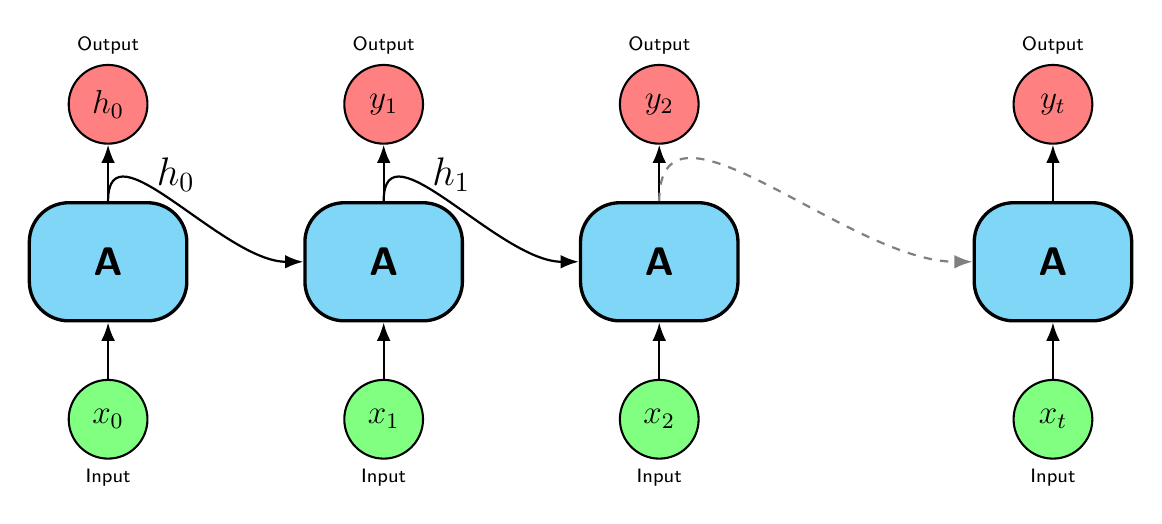
\begin{tikzpicture}[
    % GLOBAL CFG
    font=\sf \scriptsize,
    >=LaTeX,
    % Styles
    cell/.style={% For the main box
        rectangle, 
        rounded corners=5mm, 
        draw,
        very thick,
        },
    operator/.style={%For operators like +  and  x
        circle,
        draw,
        inner sep=-0.5pt,
        minimum height =.2cm,
        },
    function/.style={%For functions
        ellipse,
        draw,
        inner sep=1pt
        },
    ct/.style={% For external inputs and outputs
        circle,
        draw,
        line width = .75pt,
        minimum width=1cm,
        inner sep=1pt,
        },
    gt/.style={% For internal inputs
        rectangle,
        draw,
        minimum width=4mm,
        minimum height=3mm,
        inner sep=1pt
        },
    mylabel/.style={% something new that I have learned
        font=\scriptsize\sffamily
        },
    ArrowC1/.style={% Arrows with rounded corners
        rounded corners=.25cm,
        thick,
        },
    ArrowC2/.style={% Arrows with big rounded corners
        rounded corners=.5cm,
        thick,
        },
    ]

%Start drawing the thing...    
    % Draw the cell: 
    \node [cell, minimum height =1.5cm, minimum width=2cm, fill=cyan!50] (first) at (-1.0, 0){\Large \textbf{A}}; 
    \node [cell, minimum height =1.5cm, minimum width=2cm, fill=cyan!50] (second) at (2.5, 0){\Large \textbf{A}};
    \node [cell, minimum height =1.5cm, minimum width=2cm, fill=cyan!50] (third) at (6,0){\Large \textbf{A}};
    \node [cell, minimum height =1.5cm, minimum width=2cm, fill=cyan!50] (fourth) at (11,0){\Large \textbf{A}};

% Start connecting all.
    %Intersections and displacements are used. 
    % Drawing arrows    
    %\draw [->, ArrowC1] (first) -- (second);
    %\draw [->, ArrowC1] (second) -- (third);
    %\draw [->, ArrowC1] (third) -- (fourth);
    %\draw [->, ArrowC1] (first) -- (second);

    %\node[ct, label={[mylabel]Cell state}] (c) at (-4,1.5) {\empt{c}{t-1}};
    \node[ct, label={[mylabel]Output}, fill = red!50] (h) at (-1, 2) {\large $h_{0}$}; % , fill=blue
    \node[ct, label={[mylabel]below:Input}, fill = green!50] (x) at (-1, -2) {\large $x_0$}; %, fill = magenta
    \draw [->, ArrowC1] (x) -- (first);
    \draw [->, ArrowC1] (first) -- (h);

    %\draw [->, ArrowC1] (first -| first)++(1.5,0) -| (first); 
    %\draw [->, ArrowC1] (h -| ht)++(-0.5,0) -| (ht);
    %\draw [->, ArrowC1] (h -| ht)++(-0.5,0) -| (ht);
    %\draw [->, ArrowC1] (h -| ht)++(-0.5,0) -| (ht);
    
    \node[ct, label={[mylabel]Output}, fill = red!50] (h2) at (2.5, 2) {\large $y_{1}$};
    \node[ct, label={[mylabel]below:Input}, fill = green!50] (x2) at (2.5, -2) {\large $x_1$};
    \draw [->, ArrowC1] (x2) -- (second);
    \draw [->, ArrowC1] (second) -- (h2);
    
    \node[ct, label={[mylabel]Output},  fill = red!50] (h3) at (6, 2) {\large $y_{2}$};
    \node[ct, label={[mylabel]below:Input}, fill = green!50] (x3) at (6, -2) {\large $x_2$};
    \draw [->, ArrowC1] (x3) -- (third);
    \draw [->, ArrowC1] (third) -- (h3);
    
    \node[ct, label={[mylabel]Output},  fill = red!50] (ht) at (11, 2) {\large $y_{t}$};
    \node[ct, label={[mylabel]below:Input}, fill = green!50] (xt) at (11 , -2) {\large $x_t$};
    \draw [->, ArrowC1] (xt) -- (fourth);
    \draw [->, ArrowC1] (fourth) -- (ht);  
    
    \path[->, thick, black] (first) edge [out=90, in=180] node[above, midway] {\Large $h_0$} (second) ;
    \path[->, thick, black] (second) edge [out=90, in=180] node[above, midway] {\Large $h_1$} (third);
    \path[->, thick, gray, dashed] (third) edge [out=90, in=180] node[above, midway] {} (fourth);
    %\path[->, thick, black] (third) edge [out=90, in=180] (fourth);
    
    %\draw (first) to [out=0, in=0,looseness=8] (first);
    \end{tikzpicture}
    
    \caption{Unrolling Figuere \ref{fig:rnn} in time yields this structure. Inpired by \href{http://colah.github.io/posts/2015-08-Understanding-LSTMs/}{http://colah.github.io/posts/2015-08-Understanding-LSTMs/}.}
    \label{fig:rnn_unrolled}
\end{figure}
That might be more clear from figure \ref{fig:rnn_unrolled} shows the recurrent network unrolled in time. The way of structuring it resembles the earlier structures discussed in Section \ref{sec:artificial neural networks}. The connection between the nodes %in this kind of networks 
are a directed graph along a temporal sequence. The hidden from the previous step is fed into the next. $h_0$ is only dependant on $x_0$, while $h_t$ is dependant on $x_0, x_1, \cdots, x_t $. This example shows a one layer recurrent network. All time steps are passed through the same node. The RNN reuse the weights on the input and hidden states for all time steps. Let t denotes the length of the training sequence. The "memory" stores the useful information from $x_0, x_1, \cdots, x_t $ needed to make a prediction. Performing the same task on all inputs along the sequence. This reduces the complexity of parameters and in turn reducing the risk of overfitting. Obtaining a more general relation between input and output.
% It is used to predict the next word in a sentence or the next tone in a song.  
%%%%%%%%%%%%%%%%%%%%%%%%%%%%%%%%%%%%%%%%%%%%%%%%%%%%%%%%%%%%%%%%%%%%%%%%%%%%%%%%%%%%%
Learning long term dependencies can be a challenging. Learning is done by backpropagating the error signal thought the network. For more details see Section \ref{sec:backprop_learning_algorithm}. Working with longer sequences the error signal tend to blow up or vanish. Exploding gradients can cause the weights to oscillate. Learning from small or vanishing gradients takes ages, or might not learn anything at all. More advanced forms of recurrent nets control the information flow using gates. \textbf{cite 1997 and cite 1999 learning to forget.}

\subsubsection{Long Short-term memory network, LSTM} \label{sec:lstm}
%\textbf{Use recurrent self-connections instead of loops} \textcolor{red}{Ufullstendig setning}. 
The memory unit introduced by Sepp Hochreiter and Jürgen Schmidhuber in 1997 set performance records in multiple domains. The paper introduces gates to regulate the flow of information. A gate is structure that can be opened or closed. Having values in the range zero to one, it truncate the noise signal from the input and the output. They propose an approach for constant error flow in order to alleviate the issues with exploding or vanishing gradients. The original memory cell contains input and output gates. Gers et. al. 1999 proposed to add an additional gate, the forget gate. The idea was to enable the LSTM to reset its own memory. Resetting the memory releases internal resources and enable you to learn even more.

Because of the interdisciplinary nature of this thesis this section provides a comprehensive walk through the LSTM cell and its relevant equations. The memory unit is displayed in Figure \ref{fig:lstm_unit}. The legend describing the different components of the computational graph is available in Figure \ref{fig:legend_lstm}. The information flow thought the cell is regulated by three gates; the forget gate, the input gate and the output gate. These gates are neural networks. The forget gate learn what part of the cell state (the long-term memory) it should forget. The input gate learns the information from the input it should add to the cell state. The output gate learns which information it should send to the output. The process of training is repeated until the network reaches an acceptable performance. In other words \textit{the extent to which this potential can be exploited is limited to the effectiveness of the training procedure applied}. 
% Attempt to explain the figures.

There is two types of techniques involved in the training procedure, forward- and backward pass. \textit{For each training instance, the algorithm feeds it to the network and computes the output of every neuron in each consecutive layer (this is the forward pass, just as when making a prediction).} %A forward pass propagates the input trough the network. In the same way you would make a prediction. 
The error signal is the different between the true and the predicted values. The learning algorithm involves backpropagating the error signal in order to compute a suitable adjustment of the weights. For this particular architecture, LSTM, the gates are trained neural network. Learning which information to let thought the gate.
% More details concerning gradient based learning in Section \ref{sec:backprop_learning_algorithm}.
% Introducing some terminology, a prediction is the result of forward passing the information through the network. 

\subsubsection{Feed forward} \label{sec:forward_pass_lstm}
\begin{figure*}[hp]
             \begin{subfigure}[b]{\textwidth}   
            \centering 
            
    
    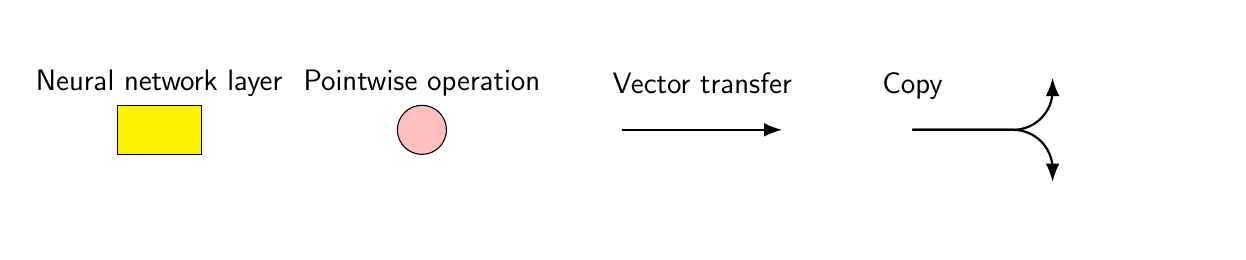
\begin{tikzpicture}[ % GLOBAL CFG
    font=\sf \scriptsize,
    >=LaTeX,
    scale = 0.89,
    every node/.style={scale=0.89},
    % Styles
    cell/.style={% For the main box
        rectangle, 
        rounded corners=5mm, 
        draw,
        very thick,
        },
    operator/.style={%For operators like +  and  x
        circle,
        draw,
        inner sep=-0.5pt,
        minimum height =.70cm,
        },
    function/.style={%For functions
        ellipse,
        draw,
        inner sep=1pt
        },
    ct/.style={% For external inputs and outputs
        circle,
        draw,
        line width = .75pt,
        minimum width=1cm,
        inner sep=1pt,
        },
    gt/.style={% For internal inputs
        rectangle,
        draw,
        minimum width=12mm,
        minimum height=7mm,
        inner sep=1pt
        },
    mylabel/.style={% something new that I have learned
        font=\scriptsize\sffamily ,
        opacity = 0.2, 
        size = \large,
        },
    ArrowC1/.style={% Arrows with rounded corners
        rounded corners=10cm,
        thick,
        },
    ArrowC2/.style={% Arrows with big rounded corners
        rounded corners=.5cm,
        thick,
        },
    ]
    
    \node [gt, fill = yellow, opacity = 1.0, label = {\large Neural network  layer}] (ibox4) at (-2.75, 0) {}; 
    \node [operator, fill = pink, opacity = 1.0, label = {\large Pointwise operation}] (mux1) at (1, 0) { }; 
    
    % Vector transfer element
    \node [operator, fill = pink, opacity = .0] (n1) at (3.5, 0) { }; 
    \node [operator, fill = pink, opacity = .0] (n2) at (6.5, 0) { }; 
    \draw [->, ArrowC2, opacity = 1.0] (n1) -- (n2) node[midway, above=3.5mm of n1] {\large Vector transfer};
    
    % copy
    \node [operator, fill = pink, opacity = .0] (c1) at (10, 1.1) { }; 
    \node [operator, fill = pink, opacity = .0] (c2) at (10, -1.1) { };
    \node [operator, fill = pink, opacity = .0] (c3) at (8, 0) { }; 
    
    \draw [->, ArrowC2, opacity = 1.0] (c3 -| c1)++(-2., 0) -| (c1) node[above=-0.5mm of c3] {\large Copy};
    \draw [->, ArrowC2, opacity = 1.0] (c3 -| c2)++(-2., 0) -| (c2) ;

    % Concatenate
    \node [operator, fill = pink, opacity = .0] (co1) at (10, 1.0) { }; 
    \node [operator, fill = pink, opacity = .0] (co2) at (10, -1.0) { };
    \node [operator, fill = pink, opacity = .0] (co3) at (12, 0) { }; 
    
    %\draw [->, ArrowC2, opacity = 1.0, label = {Vector Transfer}] (c1) -- (c3) ;
    %\draw [->, ArrowC2, opacity = 1.0, label = {Vector Transfer}] (c1 -| c3)++(.5, 3.5) -| (c1) ;

    %\draw [->, ArrowC2, opacity = 1.0] (co1) |- (co3); %(co1) -- (co3);
    %\draw [->, ArrowC2, opacity = 1.0] (co2) |- (co3) node[above=0.5mm of co3] {\large Concatenate};
    
    \end{tikzpicture}
    
    
    


            \caption{Legend.}
            \label{fig:legend_lstm}
        \end{subfigure}
        \vskip\baselineskip
        \begin{subfigure}[b]{0.475\textwidth}   
            \centering 
            
% used to avoid putting the same thing several times...
% Command \empt{var1}{var2}
    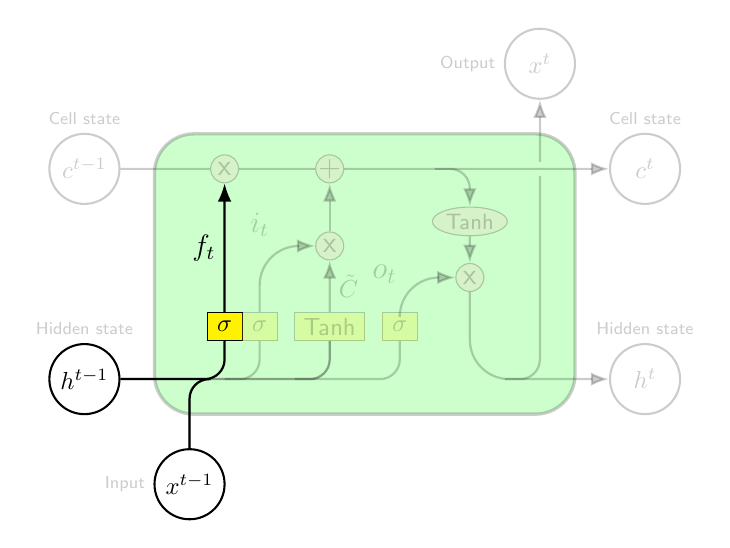
\begin{tikzpicture}[
    % GLOBAL CFG
    font=\sf \scriptsize,
    >=LaTeX,
    scale = 0.89,
    every node/.style={scale=0.89},
    % Styles
    cell/.style={% For the main box
        rectangle, 
        rounded corners=5mm, 
        draw,
        very thick,
        },
    operator/.style={%For operators like +  and  x
        circle,
        draw,
        inner sep=-0.5pt,
        minimum height =.4cm,
        },
    function/.style={%For functions
        ellipse,
        draw,
        inner sep=1pt
        },
    ct/.style={% For external inputs and outputs
        circle,
        draw,
        line width = .75pt,
        minimum width=1cm,
        inner sep=1pt,
        },
    gt/.style={% For internal inputs
        rectangle,
        draw,
        minimum width=5mm,
        minimum height=4mm,
        inner sep=1pt
        },
    mylabel/.style={% something new that I have learned
        font=\scriptsize\sffamily ,
        opacity = 0.2]
        },
    ArrowC1/.style={% Arrows with rounded corners
        rounded corners=.25cm,
        thick,
        },
    ArrowC2/.style={% Arrows with big rounded corners
        rounded corners=.5cm,
        thick,
        },
    ]

%Start drawing the thing...    
    % Draw the cell: 
    \node [cell, minimum height =4cm, minimum width=6cm, fill = green
    , opacity=0.2] at (0,0){} ;

    % Draw inputs named ibox#
    \node [gt, fill = yellow, opacity = 1.] (ibox1) at (-2,-0.75) {\normalsize $\sigma$}; % first sigma
    \node [gt, fill = yellow, opacity = 0.2] (ibox2) at (-1.5,-0.75) {\normalsize $\sigma$}; % second sigma
    \node [gt, minimum width=1cm, fill = yellow, opacity = 0.2] (ibox3) at (-0.5,-0.75) {\normalsize Tanh}; % 
    \node [gt, fill = yellow, opacity = 0.2] (ibox4) at (0.5,-0.75) {\normalsize $\sigma$};

    % Draw opérators   named mux# , add# and func# 
    % $\times$ istenfor x?
    \node [operator, fill = pink, opacity = 0.2] (mux1) at (-2,1.5) {\large x}; % cell state x
    \node [operator, fill = pink, opacity = 0.2] (add1) at (-0.5,1.5) {\large +}; % cell state +
    \node [operator, fill = pink, opacity = 0.2] (mux2) at (-0.5,0.4) {\large x}; %  (-0.5,0)
    \node [operator, fill = pink, opacity = 0.2] (mux3) at (1.5,-0.05) {\large x};
    \node [function, fill = pink, opacity = 0.2] (func1) at (1.5,0.75) {\small Tanh};

    % Draw External inputs? named as basis c,h,x
    %\node[ct, label={[mylabel]Cell state}] (c) at (-4,1.5) {\empt{c}{t-1}};
    %\node[ct, label={[mylabel]Hidden state}, fill = purple, opacity =0.3] (h) at (-4,-1.5) {\empt{h}{t-1}};
    %\node[ct, label={[mylabel]left:Input}, fill = blue, opacity =0.3] (x) at (-2.5,-3) {\empt{x}{t}};
    
    % Removed labels , fill = purple, opacity =0.3
    \node[ct, label={[mylabel]Cell state}, opacity = 0.2] (c) at (-4,1.5) {\normalsize $c^{t-1}$};
    \node[ct, label={[mylabel]Hidden state}, opacity = 1.] (h) at (-4,-1.5) {\normalsize $h^{t-1}$};
    \node[ct, label={[mylabel]left:Input}, opacity = 1.0] (x) at (-2.5,-3) {\normalsize $x^{t-1}$};

    % Draw External outputs? named as basis c2,h2,x2
    \node[ct, label={[mylabel]Cell state}, opacity = 0.2] (c2) at (4,1.5) {\normalsize $c^{t}$};
    \node[ct, label={[mylabel]Hidden state}, opacity = 0.2] (h2) at (4,-1.5) {\normalsize $h^{t}$};
    \node[ct, label={[mylabel]left:Output}, opacity = 0.2] (x2) at (2.5,3) {\normalsize $x^{t}$};
    
    % Start connecting all.
    
    % Intersections and displacements are used. 
    % Drawing arrows    
    \draw [->, ArrowC1, opacity = 0.2] (c) -- (mux1) -- (add1) -- (c2);

    % Inputs
    \draw [ArrowC1, opacity = 0.2] (h) -| (ibox4) ;
    \draw [ArrowC1] (h) -| (ibox1)  ; % to sigmoid
    \draw [ArrowC1, opacity = 1.0] (x -| h2)++(-6.2, 1.5) -| (x); % input to first sigmoid

    \draw [ArrowC1, opacity = 0.2] (h -| ibox2)++(-0.5,0) -| (ibox2); % to second sigmoid
    \draw [ArrowC1, opacity = 0.2] (h -| ibox3)++(-0.5,0) -| (ibox3); % to tanh
    \draw [ArrowC1, opacity = 0.2] (x) -- (x |- h)-| (ibox3); % inout to tanh
    

    % Internal - possibility , rotate = 90
    \draw [->, ArrowC2, opacity = 1.] (ibox1) -- (mux1) node[midway, left] {\large $f_t$};
    \draw [->, ArrowC2, opacity = 0.2] (ibox2) |- (mux2) node[midway, above] {\large $i_t$};
    \draw [->, ArrowC2, opacity = 0.2] (ibox3) -- (mux2) node[midway, right] {\normalsize $\Tilde{C}$};
    \draw [->, ArrowC2, opacity = 0.2] (ibox4) |- (mux3);
    \draw [->, ArrowC2, opacity = 0.2] (mux2) -- (add1);
    \draw [->, ArrowC1, opacity = 0.2] (add1 -| func1)++(-0.5,0) -| (func1); % node[midway, above] {d};
    \draw [->, ArrowC2, opacity = 0.2] (func1) -- (mux3) ;

    %Outputs
    \draw [->, ArrowC2, opacity=0.2] (mux3) |- (h2) ;
    \draw (c2 -| x2) ++(0,-0.1) coordinate (i1) node[midway, right, opacity=0.2] {\Large $o_t$};
    \draw [-, ArrowC1, opacity=0.2] (h2 -| x2)++(-0.5,0) -| (i1);
    \draw [->, ArrowC2, opacity=0.2] (i1)++(0,0.2) -- (x2) ;
    %\node [cell, minimum height =4cm, minimum width=6cm, fill = pink, opacity=.8] at (0,0){\Large A} ;
    
    %\node [cell, minimum height =4cm, minimum width=6cm, fill = green
    %, opacity=0.2] at (0,0){} ;
    
\end{tikzpicture}


            \caption[something]
            {{\small   The forget gate: $f_t = \sigma \left(W_f\dot \left[h_{t-h}, x{t} \right] + b_f \right)$ 
            \\ \\ \color{white}{ooooooooooooooooooooooooo} }}

            \label{fig:forget_gate}
        \end{subfigure}
        \quad
        \begin{subfigure}[b]{0.475\textwidth}   
            \centering 
            % By J. Leon, Beerware licence is acceptable...
% https://tex.stackexchange.com/questions/432312/how-do-i-draw-an-lstm-cell-in-tikz?rq=1

% used to avoid putting the same thing several times...
% Command \empt{var1}{var2}
    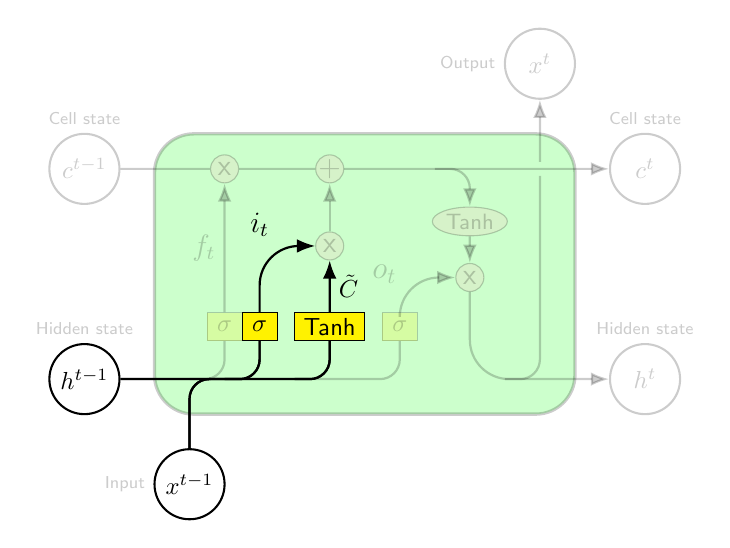
\begin{tikzpicture}[
    % GLOBAL CFG
    font=\sf \scriptsize,
    >=LaTeX,
    scale = 0.89,
    every node/.style={scale=0.89},
    % Styles
    cell/.style={% For the main box
        rectangle, 
        rounded corners=5mm, 
        draw,
        very thick,
        },
    operator/.style={%For operators like +  and  x
        circle,
        draw,
        inner sep=-0.5pt,
        minimum height =.4cm,
        },
    function/.style={%For functions
        ellipse,
        draw,
        inner sep=1pt
        },
    ct/.style={% For external inputs and outputs
        circle,
        draw,
        line width = .75pt,
        minimum width=1cm,
        inner sep=1pt,
        },
    gt/.style={% For internal inputs
        rectangle,
        draw,
        minimum width=5mm,
        minimum height=4mm,
        inner sep=1pt
        },
    mylabel/.style={% something new that I have learned
        font=\scriptsize\sffamily ,
        opacity = 0.2]
        },
    ArrowC1/.style={% Arrows with rounded corners
        rounded corners=.25cm,
        thick,
        },
    ArrowC2/.style={% Arrows with big rounded corners
        rounded corners=.5cm,
        thick,
        },
    ]

%Start drawing the thing...    
    % Draw the cell: 
    \node [cell, minimum height =4cm, minimum width=6cm, fill = green
    , opacity=0.2] at (0,0){} ;

    % Draw inputs named ibox#
    \node [gt, fill = yellow, opacity = 0.2] (ibox1) at (-2,-0.75) {\normalsize $\sigma$}; % first sigma
    \node [gt, fill = yellow, opacity = 1.0] (ibox2) at (-1.5,-0.75) {\normalsize $\sigma$}; % second sigma
    \node [gt, minimum width=1cm, fill = yellow, opacity = 1.0] (ibox3) at (-0.5,-0.75) {\normalsize Tanh}; % 
    \node [gt, fill = yellow, opacity = 0.2] (ibox4) at (0.5,-0.75) {\normalsize $\sigma$}; % last sigmoid

    % Draw opérators   named mux# , add# and func# 
    % $\times$ istenfor x?
    \node [operator, fill = pink, opacity = 0.2] (mux1) at (-2,1.5) {\large x}; % cell state x
    \node [operator, fill = pink, opacity = 0.2] (add1) at (-0.5,1.5) {\large +}; % cell state +
    \node [operator, fill = pink, opacity = 0.2] (mux2) at (-0.5,0.4) {\large x}; %  (-0.5,0)
    \node [operator, fill = pink, opacity = 0.2] (mux3) at (1.5,-0.05) {\large x};
    \node [function, fill = pink, opacity = 0.2] (func1) at (1.5,0.75) {\small Tanh};

    % Draw External inputs? named as basis c,h,x
    %\node[ct, label={[mylabel]Cell state}] (c) at (-4,1.5) {\empt{c}{t-1}};
    %\node[ct, label={[mylabel]Hidden state}, fill = purple, opacity =0.3] (h) at (-4,-1.5) {\empt{h}{t-1}};
    %\node[ct, label={[mylabel]left:Input}, fill = blue, opacity =0.3] (x) at (-2.5,-3) {\empt{x}{t}};
    
    % Removed labels , fill = purple, opacity =0.3
    \node[ct, label={[mylabel]Cell state}, opacity = 0.2] (c) at (-4,1.5) {\normalsize $c^{t-1}$};
    \node[ct, label={[mylabel]Hidden state}, opacity = 1.] (h) at (-4,-1.5) {\normalsize $h^{t-1}$};
    %\node[ct, label={[mylabel]left:Output}, opacity = 1.0] (x) at (-2.5,-3) {\normalsize $x^{t}$};
    \node[ct, label={[mylabel]left:Input}, opacity = 1.] (x) at (-2.5,-3) {\normalsize $x^{t-1}$};

    % Draw External outputs? named as basis c2,h2,x2
    \node[ct, label={[mylabel]Cell state}, opacity = 0.2] (c2) at (4,1.5) {\normalsize $c^{t}$};
    \node[ct, label={[mylabel]Hidden state}, opacity = 0.2] (h2) at (4,-1.5) {\normalsize $h^{t}$};
    \node[ct, label={[mylabel]left:Output}, opacity = 0.2] (x2) at (2.5,3) {\normalsize $x^{t}$};
    
    % Start connecting all.
    
    % Intersections and displacements are used. 
    % Drawing arrows    
    \draw [->, ArrowC1, opacity = 0.2] (c) -- (mux1) -- (add1) -- (c2);

    % Inputs
    \draw [ArrowC1, opacity = 0.2] (h) -| (ibox4) ;
    \draw [ArrowC1] (h) -| (ibox2)  ; % to second sigmoid
    \draw [ArrowC1, opacity = .2] (h -| ibox1)++(-0.5,0) -| (ibox1); % to second sigmoid

    \draw [ArrowC1, opacity = 1.2] (x -| h2)++(-6.2, 1.5) -| (x); % input to first sigmoid

    \draw [ArrowC1, opacity = 1.0] (h -| ibox2)++(-0.5,0) -| (ibox2); % to second sigmoid
    \draw [ArrowC1, opacity = 1.0] (h -| ibox3)++(-0.5,0) -| (ibox3); % to tanh
    \draw [ArrowC1, opacity = 1.] (x) -- (x |- h)-| (ibox3); % inout to tanh

    % Internal - possibility , rotate = 90
    \draw [->, ArrowC2, opacity = 0.2] (ibox1) -- (mux1) node[midway, left] {\large $f_t$};
    \draw [->, ArrowC2, opacity = 1.0] (ibox2) |- (mux2) node[midway, above] {\large $i_t$};
    \draw [->, ArrowC2, opacity = 1.0] (ibox3) -- (mux2) node[midway, right] {\normalsize $\Tilde{C}$};
    \draw [->, ArrowC2, opacity = 0.2] (ibox4) |- (mux3);
    \draw [->, ArrowC2, opacity = 0.2] (mux2) -- (add1);
    \draw [->, ArrowC1, opacity = 0.2] (add1 -| func1)++(-0.5,0) -| (func1); % node[midway, above] {d};
    \draw [->, ArrowC2, opacity = 0.2] (func1) -- (mux3) ;

    %Outputs
    \draw [->, ArrowC2, opacity=0.2] (mux3) |- (h2) ;
    \draw (c2 -| x2) ++(0,-0.1) coordinate (i1) node[midway, right, opacity=0.2] {\Large $o_t$};
    \draw [-, ArrowC1, opacity=0.2] (h2 -| x2)++(-0.5,0) -| (i1);
    \draw [->, ArrowC2, opacity=0.2] (i1)++(0,0.2) -- (x2) ;
    %\node [cell, minimum height =4cm, minimum width=6cm, fill = pink, opacity=.8] at (0,0){\Large A} ;
    
    %\node [cell, minimum height =4cm, minimum width=6cm, fill = green
    %, opacity=0.2] at (0,0){} ;
    
\end{tikzpicture}


            \caption[]
            {{\small Candidate information: $\Tilde{C_t} = tanh \left( W_C \dot \left[ h_{t-1}, x_t \right] + b_C \right)$  } \\ \\  The input gate: $i_t = \sigma \left( W_i \dot \left[ h_{t-1}, x_t \right] + b_i \right)$}

            \label{fig:input_gate}
        \end{subfigure}
                \begin{subfigure}[b]{0.475\textwidth}   
            \centering 
            % By J. Leon, Beerware licence is acceptable...
% https://tex.stackexchange.com/questions/432312/how-do-i-draw-an-lstm-cell-in-tikz?rq=1

% used to avoid putting the same thing several times...
% Command \empt{var1}{var2}
    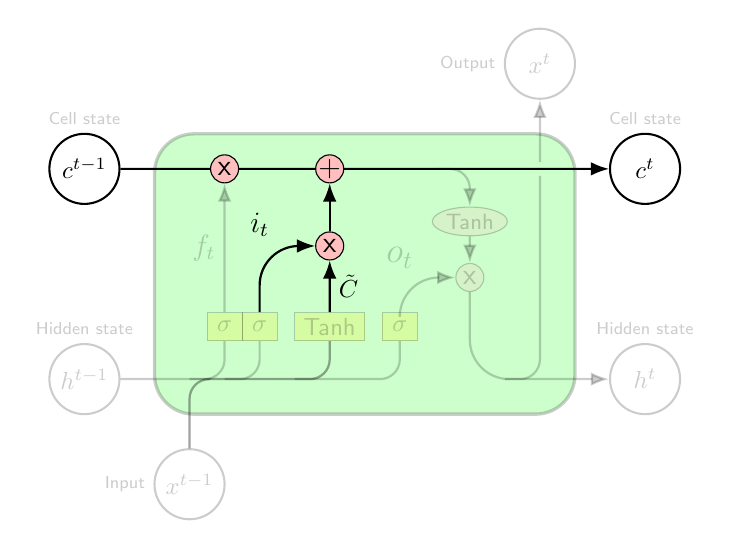
\begin{tikzpicture}[
    % GLOBAL CFG
    font=\sf \scriptsize,
    >=LaTeX,
    scale = 0.89,
    every node/.style={scale=0.89},
    % Styles
    cell/.style={% For the main box
        rectangle, 
        rounded corners=5mm, 
        draw,
        very thick,
        },
    operator/.style={%For operators like +  and  x
        circle,
        draw,
        inner sep=-0.5pt,
        minimum height =.4cm,
        },
    function/.style={%For functions
        ellipse,
        draw,
        inner sep=1pt
        },
    ct/.style={% For external inputs and outputs
        circle,
        draw,
        line width = .75pt,
        minimum width=1cm,
        inner sep=1pt,
        },
    gt/.style={% For internal inputs
        rectangle,
        draw,
        minimum width=5mm,
        minimum height=4mm,
        inner sep=1pt
        },
    mylabel/.style={% something new that I have learned
        font=\scriptsize\sffamily ,
        opacity = 0.2]
        },
    ArrowC1/.style={% Arrows with rounded corners
        rounded corners=.25cm,
        thick,
        },
    ArrowC2/.style={% Arrows with big rounded corners
        rounded corners=.5cm,
        thick,
        },
    ]

%Start drawing the thing...    
    % Draw the cell: 
    \node [cell, minimum height =4cm, minimum width=6cm, fill = green
    , opacity=0.2] at (0,0){} ;

    % Draw inputs named ibox#
    \node [gt, fill = yellow, opacity = 0.2] (ibox1) at (-2,-0.75) {\normalsize $\sigma$}; % first sigma
    \node [gt, fill = yellow, opacity = 0.2] (ibox2) at (-1.5,-0.75) {\normalsize $\sigma$}; % second sigma
    \node [gt, minimum width=1cm, fill = yellow, opacity = .2] (ibox3) at (-0.5,-0.75) {\normalsize Tanh}; % 
    \node [gt, fill = yellow, opacity = 0.2] (ibox4) at (0.5,-0.75) {\normalsize $\sigma$}; % last sigmoid

    % Draw opérators   named mux# , add# and func# 
    % $\times$ istenfor x?
    \node [operator, fill = pink, opacity = 1.0] (mux1) at (-2,1.5) {\large x}; % cell state x
    \node [operator, fill = pink, opacity = 1.0] (add1) at (-0.5,1.5) {\large +}; % cell state +
    \node [operator, fill = pink, opacity = 1.0] (mux2) at (-0.5,0.4) {\large x}; %  (-0.5,0) between input an C tilde
    \node [operator, fill = pink, opacity = 0.2] (mux3) at (1.5,-0.05) {\large x};
    \node [function, fill = pink, opacity = 0.2] (func1) at (1.5,0.75) {\small Tanh};

    % Draw External inputs? named as basis c,h,x
    %\node[ct, label={[mylabel]Cell state}] (c) at (-4,1.5) {\empt{c}{t-1}};
    %\node[ct, label={[mylabel]Hidden state}, fill = purple, opacity =0.3] (h) at (-4,-1.5) {\empt{h}{t-1}};
    %\node[ct, label={[mylabel]left:Input}, fill = blue, opacity =0.3] (x) at (-2.5,-3) {\empt{x}{t}};
    
    % Removed labels , fill = purple, opacity =0.3
    \node[ct, label={[mylabel]Cell state}, opacity = 1.0] (c) at (-4,1.5) {\normalsize $c^{t-1}$};
    \node[ct, label={[mylabel]Hidden state}, opacity = 0.2] (h) at (-4,-1.5) {\normalsize $h^{t-1}$};
    %\node[ct, label={[mylabel]left:Output}, opacity = 0.2] (x) at (-2.5,-3) {\normalsize $x^{t}$};
    \node[ct, label={[mylabel]left:Input}, opacity = 0.2] (x) at (-2.5,-3) {\normalsize $x^{t-1}$};

    % Draw External outputs? named as basis c2,h2,x2
    \node[ct, label={[mylabel]Cell state}, opacity = 1.0] (c2) at (4,1.5) {\normalsize $c^{t}$};
    \node[ct, label={[mylabel]Hidden state}, opacity = 0.2] (h2) at (4,-1.5) {\normalsize $h^{t}$};
    \node[ct, label={[mylabel]left:Output}, opacity = 0.2] (x2) at (2.5,3) {\normalsize $x^{t}$};
    
    % Start connecting all.
    
    % Intersections and displacements are used. 
    % Drawing arrows    
    \draw [->, ArrowC1, opacity = 1.0] (c) -- (mux1) -- (add1) -- (c2);

    % Inputs
    \draw [ArrowC1, opacity = .2] (h) -| (ibox4); % to first sigmoid
    %\draw [ArrowC1, opasity = 0.2] (h) -| (ibox2)  ; % to second sigmoid
    \draw [ArrowC1, opacity = .2] (h -| ibox1)++(-0.5,0) -| (ibox1); % to second sigmoid
    \draw [ArrowC1, opacity = .2] (x -| h2)++(-6.2, 1.5) -| (x); % input to first sigmoid
    \draw [ArrowC1, opacity = 0.2] (h -| ibox2)++(-0.5,0) -| (ibox2); % to second sigmoid
    \draw [ArrowC1, opacity = 0.2] (h -| ibox3)++(-0.5,0) -| (ibox3); % to tanh
    \draw [ArrowC1, opacity = 0.2] (x) -- (x |- h)-| (ibox3); % inout to tanh

    % Internal - possibility , rotate = 90
    \draw [->, ArrowC2, opacity = 0.2] (ibox1) -- (mux1) node[midway, left] {\large $f_t$};
    \draw [->, ArrowC2, opacity = 1.0] (ibox2) |- (mux2) node[midway, above] {\large $i_t$};
    \draw [->, ArrowC2, opacity = 1.0] (ibox3) -- (mux2) node[midway, right] {\normalsize $\Tilde{C}$};
    \draw [->, ArrowC2, opacity = 0.2] (ibox4) |- (mux3) node[midway, above, opacity=0.2] {\Large $o_t$}; % O_t
    \draw [->, ArrowC2, opacity = 1.0] (mux2) -- (add1);
    \draw [->, ArrowC1, opacity  = 0.2] (add1 -| func1)++(-0.5,0) -| (func1); % node[midway, above] {d};
    \draw [->, ArrowC2, opacity = 0.2] (func1) -- (mux3) ;

    %Outputs
    \draw [->, ArrowC2, opacity=0.2] (mux3) |- (h2) ;
    \draw (c2 -| x2) ++(0,-0.1) coordinate (i1);
    \draw [-, ArrowC1, opacity=0.2] (h2 -| x2)++(-0.5,0) -| (i1);
    \draw [->, ArrowC2, opacity=0.2] (i1)++(0,0.2) -- (x2) ;
    %\node [cell, minimum height =4cm, minimum width=6cm, fill = pink, opacity=.8] at (0,0){\Large A} ;
    
    %\node [cell, minimum height =4cm, minimum width=6cm, fill = green
    %, opacity=0.2] at (0,0){} ;
    
\end{tikzpicture}


            \caption[something]%
            {{\small Updating the cell state, $C_t = f_t * C_{t-1} + i_t*\Tilde{C_t}$ \\ \\ \color{white}{ooooooooooooooooooooooooo}}}

            \label{fig:update_memory}
        \end{subfigure}
        \quad
        \begin{subfigure}[b]{0.475\textwidth}   
            \centering 
            
% used to avoid putting the same thing several times...
% Command \empt{var1}{var2}
    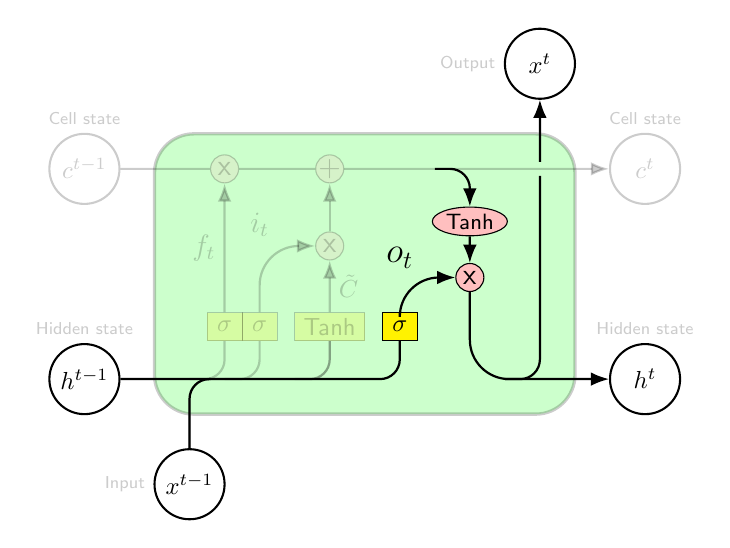
\begin{tikzpicture}[
    % GLOBAL CFG
    font=\sf \scriptsize,
    >=LaTeX,
    scale = 0.89,
    every node/.style={scale=0.89},
    % Styles
    cell/.style={% For the main box
        rectangle, 
        rounded corners=5mm, 
        draw,
        very thick,
        },
    operator/.style={%For operators like +  and  x
        circle,
        draw,
        inner sep=-0.5pt,
        minimum height =.4cm,
        },
    function/.style={%For functions
        ellipse,
        draw,
        inner sep=1pt
        },
    ct/.style={% For external inputs and outputs
        circle,
        draw,
        line width = .75pt,
        minimum width=1cm,
        inner sep=1pt,
        },
    gt/.style={% For internal inputs
        rectangle,
        draw,
        minimum width=5mm,
        minimum height=4mm,
        inner sep=1pt
        },
    mylabel/.style={% something new that I have learned
        font=\scriptsize\sffamily ,
        opacity = 0.2]
        },
    ArrowC1/.style={% Arrows with rounded corners
        rounded corners=.25cm,
        thick,
        },
    ArrowC2/.style={% Arrows with big rounded corners
        rounded corners=.5cm,
        thick,
        },
    ]

%Start drawing the thing...    
    % Draw the cell: 
    \node [cell, minimum height =4cm, minimum width=6cm, fill = green
    , opacity=0.2] at (0,0){} ;

    % Draw inputs named ibox#
    \node [gt, fill = yellow, opacity = 0.2] (ibox1) at (-2,-0.75) {\normalsize $\sigma$}; % first sigma
    \node [gt, fill = yellow, opacity = 0.2] (ibox2) at (-1.5,-0.75) {\normalsize $\sigma$}; % second sigma
    \node [gt, minimum width=1cm, fill = yellow, opacity = .2] (ibox3) at (-0.5,-0.75) {\normalsize Tanh}; % 
    \node [gt, fill = yellow, opacity = 1.0] (ibox4) at (0.5,-0.75) {\normalsize $\sigma$}; % last sigmoid

    % Draw opérators   named mux# , add# and func# 
    % $\times$ istenfor x?
    \node [operator, fill = pink, opacity = 0.2] (mux1) at (-2,1.5) {\large x}; % cell state x
    \node [operator, fill = pink, opacity = 0.2] (add1) at (-0.5,1.5) {\large +}; % cell state +
    \node [operator, fill = pink, opacity = 0.2] (mux2) at (-0.5,0.4) {\large x}; %  (-0.5,0) between input an C tilde
    \node [operator, fill = pink, opacity = 1.0] (mux3) at (1.5,-0.05) {\large x};
    \node [function, fill = pink, opacity = 1.0] (func1) at (1.5,0.75) {\small Tanh};

    % Draw External inputs? named as basis c,h,x
    %\node[ct, label={[mylabel]Cell state}] (c) at (-4,1.5) {\empt{c}{t-1}};
    %\node[ct, label={[mylabel]Hidden state}, fill = purple, opacity =0.3] (h) at (-4,-1.5) {\empt{h}{t-1}};
    %\node[ct, label={[mylabel]left:Input}, fill = blue, opacity =0.3] (x) at (-2.5,-3) {\empt{x}{t}};
    
    % Removed labels , fill = purple, opacity =0.3
    \node[ct, label={[mylabel]Cell state}, opacity = 0.2] (c) at (-4,1.5) {\normalsize $c^{t-1}$};
    \node[ct, label={[mylabel]Hidden state}, opacity = 1.] (h) at (-4,-1.5) {\normalsize $h^{t-1}$};
    %\node[ct, label={[mylabel]left:Output}, opacity = 1.0] (x) at (-2.5,-3) {\normalsize $x^{t}$};
    \node[ct, label={[mylabel]left:Input}, opacity = 1.0] (x) at (-2.5,-3) {\normalsize $x^{t-1}$};

    % Draw External outputs? named as basis c2,h2,x2
    \node[ct, label={[mylabel]Cell state}, opacity = 0.2] (c2) at (4,1.5) {\normalsize $c^{t}$};
    \node[ct, label={[mylabel]Hidden state}, opacity = 1.0] (h2) at (4,-1.5) {\normalsize $h^{t}$};
    \node[ct, label={[mylabel]left:Output}, opacity = 1.] (x2) at (2.5,3) {\normalsize $x^{t}$};
    
    % Start connecting all.
    
    % Intersections and displacements are used. 
    % Drawing arrows    
    \draw [->, ArrowC1, opacity = 0.2] (c) -- (mux1) -- (add1) -- (c2);

    % Inputs
    \draw [ArrowC1, opacity = 1.0] (h) -| (ibox4); % to last? sigmoid
    %\draw [ArrowC1, opasity = 0.2] (h) -| (ibox2); % to second sigmoid
    \draw [ArrowC1, opacity = 0.2] (h -| ibox1)++(-0.5,0) -| (ibox1); % to second sigmoid
    \draw [ArrowC1, opacity = 1.0] (x -| h2)++(-6.2, 1.5) -| (x); % input to first sigmoid
    \draw [ArrowC1, opacity = 0.2] (h -| ibox2)++(-0.5,0) -| (ibox2); % to second sigmoid
    \draw [ArrowC1, opacity = 0.2] (h -| ibox3)++(-0.5,0) -| (ibox3); % to tanh
    \draw [ArrowC1, opacity = 0.2] (x) -- (x |- h)-| (ibox3); % inout to tanh

    % Internal - possibility , rotate = 90
    \draw [->, ArrowC2, opacity = 0.2] (ibox1) -- (mux1) node[midway, left] {\large $f_t$};
    \draw [->, ArrowC2, opacity = 0.2] (ibox2) |- (mux2) node[midway, above] {\large $i_t$};
    \draw [->, ArrowC2, opacity = 0.2] (ibox3) -- (mux2) node[midway, right] {\normalsize $\Tilde{C}$};
    \draw [->, ArrowC2, opacity = 1.0] (ibox4) |- (mux3) node[midway, above] {\Large $o_t$}; % O_t
    \draw [->, ArrowC2, opacity = .2] (mux2) -- (add1);
    
    \draw [->, ArrowC1, opacity  = 1.0] (add1 -| func1)++(-0.5,0) -| (func1); % node[midway, above] {d};
    \draw [->, ArrowC2, opacity = 1.0] (func1) -- (mux3) ;

    %Outputs
    \draw [->, ArrowC2, opacity=1.0] (mux3) |- (h2) ;
    \draw (c2 -| x2) ++(0,-0.1) coordinate (i1);
    \draw [-, ArrowC1, opacity=1.0] (h2 -| x2)++(-0.5,0) -| (i1);
    \draw [->, ArrowC2, opacity=1.0] (i1)++(0,0.2) -- (x2) ;
    %\node [cell, minimum height =4cm, minimum width=6cm, fill = pink, opacity=.8] at (0,0){\Large A} ;
    
    %\node [cell, minimum height =4cm, minimum width=6cm, fill = green
    %, opacity=0.2] at (0,0){} ;
    
\end{tikzpicture}


            \caption[]
            {{\small The output gate: $ o_t =\sigma \left( W_o \dot \left[ h_{t-1}, x_t \right] + b_o\right) $
             \\ \\ Updating the hidden state, $ h_t = o_t*tanh\left( C_t \right)$ }}

            \label{fig:output_gate}

        \end{subfigure}

        
        
        \caption[ havner dette i figurlista ]
        {\small Walk trought the components of a LSTM and the relevant equations.
        Let t denote the time step, $\sigma$ is the activation function, $W_{\text{component}, \text{gate}}$, $H_{t}$ denotes the hidden state at time t, $C_{t}$ is the cell state at time t. Inspired by \cite{colah}. Extension of example provided by \cite{lstm_cell_tikz}.}
        \label{fig:LSTM_all}
    \end{figure*}
\begin{figure*}[hp]
        \centering
        \begin{subfigure}[b]{\textwidth}   
            \centering 
            
    
    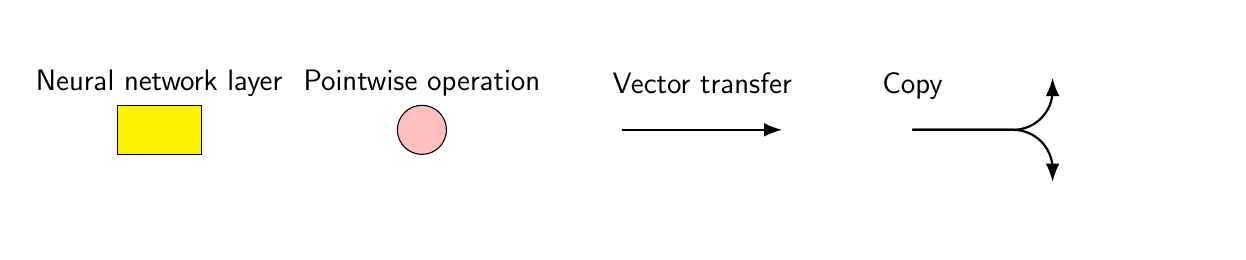
\begin{tikzpicture}[ % GLOBAL CFG
    font=\sf \scriptsize,
    >=LaTeX,
    scale = 0.89,
    every node/.style={scale=0.89},
    % Styles
    cell/.style={% For the main box
        rectangle, 
        rounded corners=5mm, 
        draw,
        very thick,
        },
    operator/.style={%For operators like +  and  x
        circle,
        draw,
        inner sep=-0.5pt,
        minimum height =.70cm,
        },
    function/.style={%For functions
        ellipse,
        draw,
        inner sep=1pt
        },
    ct/.style={% For external inputs and outputs
        circle,
        draw,
        line width = .75pt,
        minimum width=1cm,
        inner sep=1pt,
        },
    gt/.style={% For internal inputs
        rectangle,
        draw,
        minimum width=12mm,
        minimum height=7mm,
        inner sep=1pt
        },
    mylabel/.style={% something new that I have learned
        font=\scriptsize\sffamily ,
        opacity = 0.2, 
        size = \large,
        },
    ArrowC1/.style={% Arrows with rounded corners
        rounded corners=10cm,
        thick,
        },
    ArrowC2/.style={% Arrows with big rounded corners
        rounded corners=.5cm,
        thick,
        },
    ]
    
    \node [gt, fill = yellow, opacity = 1.0, label = {\large Neural network  layer}] (ibox4) at (-2.75, 0) {}; 
    \node [operator, fill = pink, opacity = 1.0, label = {\large Pointwise operation}] (mux1) at (1, 0) { }; 
    
    % Vector transfer element
    \node [operator, fill = pink, opacity = .0] (n1) at (3.5, 0) { }; 
    \node [operator, fill = pink, opacity = .0] (n2) at (6.5, 0) { }; 
    \draw [->, ArrowC2, opacity = 1.0] (n1) -- (n2) node[midway, above=3.5mm of n1] {\large Vector transfer};
    
    % copy
    \node [operator, fill = pink, opacity = .0] (c1) at (10, 1.1) { }; 
    \node [operator, fill = pink, opacity = .0] (c2) at (10, -1.1) { };
    \node [operator, fill = pink, opacity = .0] (c3) at (8, 0) { }; 
    
    \draw [->, ArrowC2, opacity = 1.0] (c3 -| c1)++(-2., 0) -| (c1) node[above=-0.5mm of c3] {\large Copy};
    \draw [->, ArrowC2, opacity = 1.0] (c3 -| c2)++(-2., 0) -| (c2) ;

    % Concatenate
    \node [operator, fill = pink, opacity = .0] (co1) at (10, 1.0) { }; 
    \node [operator, fill = pink, opacity = .0] (co2) at (10, -1.0) { };
    \node [operator, fill = pink, opacity = .0] (co3) at (12, 0) { }; 
    
    %\draw [->, ArrowC2, opacity = 1.0, label = {Vector Transfer}] (c1) -- (c3) ;
    %\draw [->, ArrowC2, opacity = 1.0, label = {Vector Transfer}] (c1 -| c3)++(.5, 3.5) -| (c1) ;

    %\draw [->, ArrowC2, opacity = 1.0] (co1) |- (co3); %(co1) -- (co3);
    %\draw [->, ArrowC2, opacity = 1.0] (co2) |- (co3) node[above=0.5mm of co3] {\large Concatenate};
    
    \end{tikzpicture}
    
    
    


            \caption{Legend for LSTM walk through.}
            \label{fig:legend_lstm}
        \end{subfigure}

        \begin{subfigure}[b]{0.475\textwidth}
            \centering
            % By J. Leon, Beerware licence is acceptable...
% https://tex.stackexchange.com/questions/432312/how-do-i-draw-an-lstm-cell-in-tikz?rq=1

% used to avoid putting the same thing several times...
% Command \empt{var1}{var2}
    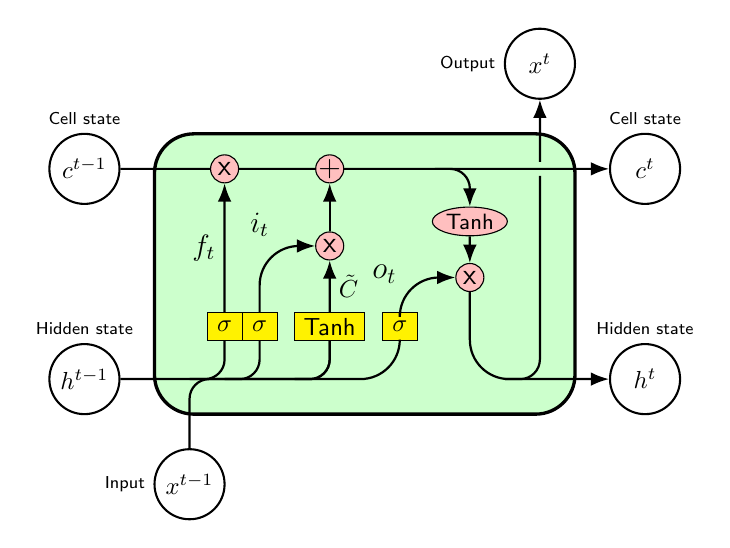
\begin{tikzpicture}[
    % GLOBAL CFG
    font=\sf \scriptsize,
    >=LaTeX,
    scale = 0.89,
    every node/.style={scale=0.89},
    % Styles
    cell/.style={% For the main box
        rectangle, 
        rounded corners=5mm, 
        draw,
        very thick,
        },
    operator/.style={%For operators like +  and  x
        circle,
        draw,
        inner sep=-0.5pt,
        minimum height =.4cm,
        },
    function/.style={%For functions
        ellipse,
        draw,
        inner sep=1pt
        },
    ct/.style={% For external inputs and outputs
        circle,
        draw,
        line width = .75pt,
        minimum width=1cm,
        inner sep=1pt,
        },
    gt/.style={% For internal inputs
        rectangle,
        draw,
        minimum width=5mm,
        minimum height=4mm,
        inner sep=1pt
        },
    mylabel/.style={% something new that I have learned
        font=\scriptsize\sffamily
        },
    ArrowC1/.style={% Arrows with rounded corners
        rounded corners=.25cm,
        thick,
        },
    ArrowC2/.style={% Arrows with big rounded corners
        rounded corners=.5cm,
        thick,
        },
    ]

%Start drawing the thing...    
    % Draw the cell: 
    \node [cell, minimum height =4cm, minimum width=6cm, fill = green!20] at (0,0){} ; % opacity=0.2

    % Draw inputs named ibox#
    \node [gt, fill = yellow] (ibox1) at (-2,-0.75) {\normalsize $\sigma$};
    \node [gt, fill = yellow] (ibox2) at (-1.5,-0.75) {\normalsize $\sigma$};
    \node [gt, minimum width=1cm, fill = yellow] (ibox3) at (-0.5,-0.75) {\normalsize Tanh};
    \node [gt, fill = yellow] (ibox4) at (0.5,-0.75) {\normalsize $\sigma$};

    % Draw opérators   named mux# , add# and func# 
    % $\times$ istenfor x?
    \node [operator, fill = pink] (mux1) at (-2,1.5) {\large x};
    \node [operator, fill = pink] (add1) at (-0.5,1.5) {\large +};
    \node [operator, fill = pink] (mux2) at (-0.5,0.4) {\large x}; %  (-0.5,0)
    \node [operator, fill = pink] (mux3) at (1.5,-0.05) {\large x};
    \node [function, fill = pink] (func1) at (1.5,0.75) {\small Tanh};

    % Draw External inputs? named as basis c,h,x
    %\node[ct, label={[mylabel]Cell state}] (c) at (-4,1.5) {\empt{c}{t-1}};
    %\node[ct, label={[mylabel]Hidden state}, fill = purple, opacity =0.3] (h) at (-4,-1.5) {\empt{h}{t-1}};
    %\node[ct, label={[mylabel]left:Input}, fill = blue, opacity =0.3] (x) at (-2.5,-3) {\empt{x}{t}};
    
    % Removed labels , fill = purple, opacity =0.3
    \node[ct, label={[mylabel]Cell state}] (c) at (-4,1.5) {\normalsize $c^{t-1}$};
    \node[ct, label={[mylabel]Hidden state}] (h) at (-4,-1.5) {\normalsize $h^{t-1}$};
    %\node[ct, label={[mylabel]left:Output}] (x) at (-2.5,-3) {\normalsize $x^{t}$};
    \node[ct, label={[mylabel]left:Input}, opacity = 1.0] (x) at (-2.5,-3) {\normalsize $x^{t-1}$};

    % Draw External outputs? named as basis c2,h2,x2
    \node[ct, label={[mylabel]Cell state}] (c2) at (4,1.5) {\normalsize $c^{t}$};
    \node[ct, label={[mylabel]Hidden state}] (h2) at (4,-1.5) {\normalsize $h^{t}$};
    \node[ct, label={[mylabel]left:Output}] (x2) at (2.5,3) {\normalsize $x^{t}$};
    
    % Start connecting all.
    
    % Intersections and displacements are used. 
    % Drawing arrows    
    \draw [->, ArrowC1] (c) -- (mux1) -- (add1) -- (c2);

    % Inputs
    \draw [ArrowC2] (h) -| (ibox4) ;
    \draw [ArrowC1] (h -| ibox1)++(-0.5,0) -| (ibox1); 
    \draw [ArrowC1] (h -| ibox2)++(-0.5,0) -| (ibox2);
    \draw [ArrowC1] (h -| ibox3)++(-0.5,0) -| (ibox3);
    \draw [ArrowC1] (x) -- (x |- h)-| (ibox3);

    % Internal - possibility , rotate = 90
    \draw [->, ArrowC2] (ibox1) -- (mux1) node[midway, left] {\large $f_t$};
    \draw [->, ArrowC2] (ibox2) |- (mux2) node[midway, above] {\large $i_t$};
    \draw [->, ArrowC2] (ibox3) -- (mux2) node[midway, right] {\normalsize $\Tilde{C}$};
    \draw [->, ArrowC2] (ibox4) |- (mux3);
    \draw [->, ArrowC2] (mux2) -- (add1);
    \draw [->, ArrowC1] (add1 -| func1)++(-0.5,0) -| (func1)  ; % node[midway, above] {d};
    \draw [->, ArrowC2] (func1) -- (mux3) ;

    %Outputs
    \draw [->, ArrowC2] (mux3) |- (h2) ;
    \draw (c2 -| x2) ++(0,-0.1) coordinate (i1) node[midway, right] {\Large $o_t$};
    \draw [-, ArrowC1, opacity=1.0] (h2 -| x2)++(-0.5,0) -| (i1);
    \draw [->, ArrowC2] (i1)++(0,0.2) -- (x2) ;
    %\node [cell, minimum height =4cm, minimum width=6cm, fill = pink, opacity=.8] at (0,0){\Large A} ;
    
\end{tikzpicture}


            \caption[Channel WV 6.2]
            {{\small Recurrent unit. LSTM cell.}}
                %\\ \\ \color{white}{ooooooooooooooooooooooooo} 
                
            \label{fig:lstm_unit}
        \end{subfigure}
        \hfill
        \begin{subfigure}[b]{0.475\textwidth}  
            \centering 
            
% used to avoid putting the same thing several times...
% Command \empt{var1}{var2}
    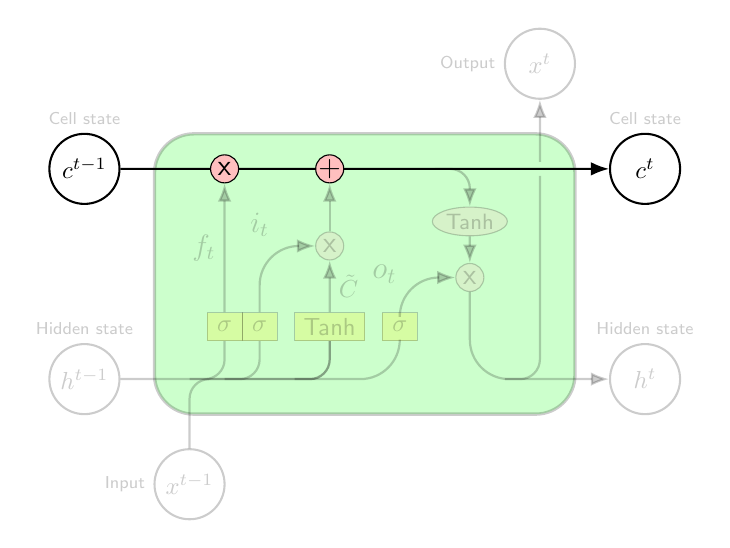
\begin{tikzpicture}[
    % GLOBAL CFG
    font=\sf \scriptsize,
    >=LaTeX,
    scale = 0.89,
    every node/.style={scale=0.89},
    % Styles
    cell/.style={% For the main box
        rectangle, 
        rounded corners=5mm, 
        draw,
        very thick,
        },
    operator/.style={%For operators like +  and  x
        circle,
        draw,
        inner sep=-0.5pt,
        minimum height =.4cm,
        },
    function/.style={%For functions
        ellipse,
        draw,
        inner sep=1pt
        },
    ct/.style={% For external inputs and outputs
        circle,
        draw,
        line width = .75pt,
        minimum width=1cm,
        inner sep=1pt,
        },
    gt/.style={% For internal inputs
        rectangle,
        draw,
        minimum width=5mm,
        minimum height=4mm,
        inner sep=1pt
        },
    mylabel/.style={% something new that I have learned
        font=\scriptsize\sffamily, 
        opacity = 0.2,
        },
    ArrowC1/.style={% Arrows with rounded corners
        rounded corners=.25cm,
        thick,
        },
    ArrowC2/.style={% Arrows with big rounded corners
        rounded corners=.5cm,
        thick,
        },
    ]

%Start drawing the thing...    
    % Draw the cell: 
    \node [cell, minimum height =4cm, minimum width=6cm, fill = green
    , opacity=0.2] at (0,0){} ;

    % Draw inputs named ibox#
    \node [gt, fill = yellow, opacity = 0.2] (ibox1) at (-2,-0.75) {\normalsize $\sigma$};
    \node [gt, fill = yellow, opacity = 0.2] (ibox2) at (-1.5,-0.75) {\normalsize $\sigma$};
    \node [gt, minimum width=1cm, fill = yellow, opacity = 0.2] (ibox3) at (-0.5,-0.75) {\normalsize Tanh};
    \node [gt, fill = yellow, opacity = 0.2] (ibox4) at (0.5,-0.75) {\normalsize $\sigma$};

    % Draw opérators   named mux# , add# and func# 
    % $\times$ istenfor x?
    \node [operator, fill = pink] (mux1) at (-2,1.5) {\large x};
    \node [operator, fill = pink] (add1) at (-0.5,1.5) {\large +};
    \node [operator, fill = pink, opacity = 0.2] (mux2) at (-0.5,0.4) {\large x}; %  (-0.5,0)
    \node [operator, fill = pink, opacity = 0.2] (mux3) at (1.5,-0.05) {\large x};
    \node [function, fill = pink, opacity = 0.2] (func1) at (1.5,0.75) {\small Tanh};

    % Draw External inputs? named as basis c,h,x
    %\node[ct, label={[mylabel]Cell state}] (c) at (-4,1.5) {\empt{c}{t-1}};
    %\node[ct, label={[mylabel]Hidden state}, fill = purple, opacity =0.3] (h) at (-4,-1.5) {\empt{h}{t-1}};
    %\node[ct, label={[mylabel]left:Input}, fill = blue, opacity =0.3] (x) at (-2.5,-3) {\empt{x}{t}};
    
    % Removed labels , fill = purple, opacity =0.3
    \node[ct, label={[mylabel]Cell state}] (c) at (-4,1.5) {\normalsize $c^{t-1}$};
    \node[ct, label={[mylabel]Hidden state}, opacity = 0.2] (h) at (-4,-1.5) {\normalsize $h^{t-1}$};
    %\node[ct, label={[mylabel]left:Output}, opacity = 0.2] (x) at (-2.5,-3) {\normalsize $x^{t}$};
    \node[ct, label={[mylabel]left:Input}, opacity = 0.2] (x) at (-2.5,-3) {\normalsize $x^{t-1}$};


    % Draw External outputs? named as basis c2,h2,x2
    \node[ct, label={[mylabel]Cell state}] (c2) at (4,1.5) {\normalsize $c^{t}$};
    \node[ct, label={[mylabel]Hidden state}, opacity = 0.2] (h2) at (4,-1.5) {\normalsize $h^{t}$};
    \node[ct, label={[mylabel]left:Output}, opacity = 0.2] (x2) at (2.5,3) {\normalsize $x^{t}$};
    
    % Start connecting all.
    
    % Intersections and displacements are used. 
    % Drawing arrows    
    \draw [->, ArrowC1] (c) -- (mux1) -- (add1) -- (c2);

    % Inputs
    \draw [ArrowC2, opacity = 0.2] (h) -| (ibox4) ;
    \draw [ArrowC1, opacity = 0.2] (h -| ibox1)++(-0.5,0) -| (ibox1); 
    \draw [ArrowC1, opacity = 0.2] (h -| ibox2)++(-0.5,0) -| (ibox2);
    \draw [ArrowC1, opacity = 0.2] (h -| ibox3)++(-0.5,0) -| (ibox3);
    \draw [ArrowC1, opacity = 0.2] (x) -- (x |- h)-| (ibox3);

    % Internal - possibility , rotate = 90
    \draw [->, ArrowC2, opacity = 0.2] (ibox1) -- (mux1) node[midway, left] {\large $f_t$};
    \draw [->, ArrowC2, opacity = 0.2] (ibox2) |- (mux2) node[midway, above] {\large $i_t$};
    \draw [->, ArrowC2, opacity = 0.2] (ibox3) -- (mux2) node[midway, right] {\normalsize $\Tilde{C}$};
    \draw [->, ArrowC2, opacity = 0.2] (ibox4) |- (mux3);
    \draw [->, ArrowC2, opacity = 0.2] (mux2) -- (add1);
    \draw [->, ArrowC1, opacity = 0.21] (add1 -| func1)++(-0.5,0) -| (func1)  ; % node[midway, above] {d};
    \draw [->, ArrowC2, opacity = 0.2] (func1) -- (mux3) ;

    %Outputs
    \draw [->, ArrowC2, opacity=0.2] (mux3) |- (h2) ;
    \draw (c2 -| x2) ++(0,-0.1) coordinate (i1) node[midway, right, opacity=0.2] {\Large $o_t$};
    \draw [-, ArrowC1, opacity=0.2] (h2 -| x2)++(-0.5,0) -| (i1);
    \draw [->, ArrowC2, opacity=0.2] (i1)++(0,0.2) -- (x2) ;
    %\node [cell, minimum height =4cm, minimum width=6cm, fill = pink, opacity=.8] at (0,0){\Large A} ;
    
    %\node [cell, minimum height =4cm, minimum width=6cm, fill = green
    %, opacity=0.2] at (0,0){} ;
    
\end{tikzpicture}


            \caption[]%
            {{\small The cell state. Keeping track of the long term dependencies.}}    
            \label{fig:cell_state_information_flow}
        \end{subfigure}

        \caption[ havner dette i figurlista ]
        {\small Walk trought the components of a LSTM and the relevant equations. Inspired by \href{https://tex.stackexchange.com/questions/432312/how-do-i-draw-an-lstm-cell-in-tikz?rq=1}{https://tex.stackexchange.com/questions/432312/how-do-i-draw-an-lstm-cell-in-tikz?rq=1} }
        \label{fig:LSTM2}
    \end{figure*}
Together Figures \ref{fig:LSTM_all} and \ref{fig:LSTM2} shows a computational graph of the LSTM unit. The relevant equations are shown in the figure text, to make it easier for the reader to follow the computations. The following subplots highlights the graphs relevant for gates and necessary calculations. %, highlighting key computations along with their respective equations. 

Figure  \ref{fig:cell_state_information_flow} shows the information flow of the cell state. Like the human brain, the LSTM cell has its own memory. The LSTM has a long term memory, known as the cell state and the short term memory referred to as the hidden state. The cell state is affected by some linear interactions, but this is very simple and the flow often remain unchanged. The hidden state is the output passed to the next cell. Structures like gates regulate the flow of information. The gates are neural networks layers with a particular activation function. It is called sigmoid function, named after the greek letter sigma, shaped like an S. Truncating the output from the gates to range between zero and one. Figure \ref{fig:activation_func_plus} shows the sigmoid and tanh functions. Zero represents a closed gate, while one describes a wide-open gate. At each time step in the sequence the LSTM receives input $x_t$ and the previous hidden state, $h_{t-1}$. These are passed trough all gates. 

% The forget gate
In order to make a prediction, one needs to feed forward information though the network. Based on the new input, the previous hidden state and the cell state, the forget gate determines which instances from the memory to remove. This is done in the forget gate shown in Figure \ref{fig:forget_gate}. Regulating the information that stays in memory frees up space, allow you to learn new things. The gate is initialized to 1, thus it can't forget anything until it has learned to forget. Exhibiting the same behavior as the original LSTM units. 

% The input gate 
Followed by determining the candidate information and filtering the input trough the input gate. Filtering in this sense refers to the component wise multiplication with a gate. This is shown in Figure \ref{fig:input_gate}.  The input gate regulates what information to store from the input. The aim of the input gate is to clean the input by reducing the noise signal. %This is done by Equations \eqref{eq:CLSTM1_input_gate} and \eqref{eq:CLSTM3_cellstate}. 
These computations are also shown in Figure \ref{fig:input_gate}.

After determining what to forget and what information to add to memory, its time to update the cell state (the long term memory). This is illustrated in Figure \ref{fig:update_memory}. At last the the hidden state (short term memory) is updated after being filtered by the output gate, see Figure \ref{fig:output_gate}. Purpose of this gate is to remove noise from the output. Preventing misrepresentations of the hidden state (short-term memory). \textbf{cite LSTM 1997} This produce the output and hidden state. Recall that sigmoid takes values in the range 0 to 1 and tangens hyperbolicus, tanh takes values between -1 and 1.

In summary, at each time step some memories are removed and others are added. The cell state is then passed through a tanh-function and filtered by the output gate. 
% \textbf{cite colah blogpost ?}
% http://colah.github.io/posts/2015-08-Understanding-LSTMs/

\subsection{Convolutional LSTM}  \label{sec:convolutional_lstm}
A variant of the LSTM network is the convolutional LSTM (ConvLSTM). First developed for precipitation nowcasting in 2015. The only difference between this and the general LSTM is that the standard fully connected neural networks (see figure \ref{fig:one_layer_mlp}) is replaced by convolutional neural network (see figure \ref{fig:convolution_padding}). This allows the LSTM network to support multi-dimensional data, capturing the spatiotemporal structure in the data. This architecture is has the potential to solve problems in time and space. 
\begin{figure}
    \centering
    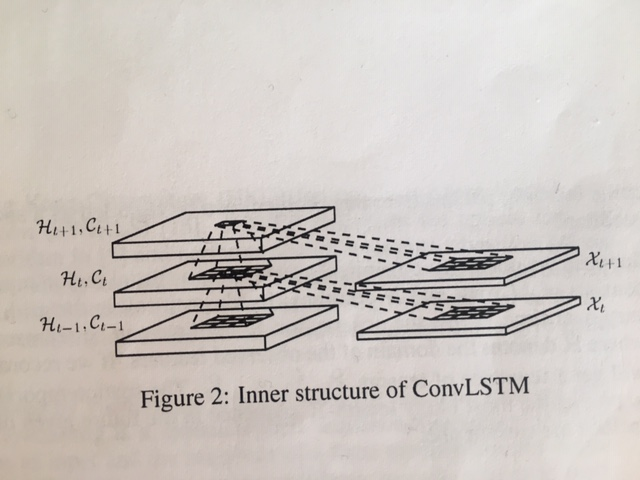
\includegraphics[scale = 0.5]{convLSTM_inside_structure.JPG}
    \caption{Structures between reccurent units in a convolutional LSTM. \textbf{Considering making this figure.} cite Conc LSTM nowcasting paper.}
    \label{fig:inside_convLSTM}
\end{figure}
Keeping the same structure as in Figure \ref{fig:lstm_unit}, while making small changes to the equations used to forward propagate the input. Equations \eqref{eq:CLSTM2_forget_gate} to \eqref{eq:CLSTM5_hidden_state} is describes the forward propagation trough a covolutional LSTM. Here $\circ$ denoted the Hademand product, which is a component wise multiplication, and * is convolution. 
%Making small adjustments to the eqations in form of componentwise multiplications instead of matrix products. Recall that a matrix product is the sum over component-wise multiplications. 
Let t denote the time step, $\sigma$ is the activation function, $tanh$ be tanges hyberbolicus, $W_{\text{component}, \text{gate}}$, $H_{t}$ denotes the hidden state at time t, $C_{t}$ is the cell state at time t. 

\begin{equation} \label{eq:CLSTM2_forget_gate}
        f_t = \sigma \left( W_{xf}*x_t + W_{hf}*H_{t-1} + W_{cf}\circ C_{t-1}+b_f \right)
\end{equation}

\begin{equation} \label{eq:CLSTM1_input_gate}
    i_t = \sigma \left( W_{xi}*x_t + W_{hi}*H_{t-1} + W_{ci}\circ C_{t-1}+b_i \right) 
\end{equation}

\begin{equation} \label{eq:CLSTM3_cellstate}
        C_t = f_t \circ C_{t-1} +i_t\circ tanh\left( W_{xc}*X_t + W_{hc}*H_{t-1} + b_c \right)
\end{equation}

\begin{equation} \label{eq:CLSTM4_output_gate}
        o_t = \sigma \left( W_{xo}*X_t + W_{ho}*H_{t-1} + W_{co}\circ C_{t}+b_o \right)
\end{equation}

\begin{equation} \label{eq:CLSTM5_hidden_state}
        H_t = o_t \circ tanh \left( C_t \right)
\end{equation}

\subsection{Padding (and Stride?)} \label{sec:padding}
% Add equation to calculate how much zero padding is needed to make a prediction of the same size.
The convolution operation shrinks the dimensions of the feature map, according to Equation \eqref{eq:output_size}. The degree of shrinking  depends on the  filter size, padding and stride. Padding zeros along the edges has an additional benefit of including the signal from the boundaries. Stride determines how far you move the filter between convolutions. In other words it control how you convolve around the input volume. Figure \ref{fig:convolution_padding} shows a example with a zero padding of one. This is sufficient to keep the input dimension using a filter of dimensions $3 \time 3$. Which can be shown by plugging the dimensions into \eqref{eq:padding_same}.

For a arbitrary image. Some definitions,
\begin{enumerate}
    \item image size, $n\times n$
    \item filter size, $f\times f$
    \item padding size, p
    \item stride, s
    \item output size, $o \times o$
\end{enumerate}

\begin{equation} \label{eq:output_size}
    o = \frac{n+2p-f}{s} + 1
\end{equation}
In some cases it can be useful to have the same shape of input and output. This is called \textit{padding same}. Solving the equation \eqref{eq:output_size} for $p$ using $o=n$ yields the following expression.
\begin{equation} \label{eq:padding_same}
    p = \frac{n\left(s-1\right)-s+f}{2}
\end{equation}

\subsection{Learning algorithm} \label{sec:backprop_learning_algorithm}
Learning is a time consuming task. The fundamental trick in deep learning is to use the performance metric as a feedback signal to adjust the weights. It adjusts in the direction of the lowest loss score for the current example (i.e. the current batch). The adjustment is the job of the optimizer, which implements backpropagation algorithmn which is the central learning algoritmn. This section aims to build a understanding of backpropagation trough time without referring to any significant mathematics. If you are interested in the mathematics behind this, read X and Y. 

\textit{Learning means finding a suitable representation of model parameters that minimize a loss function for a given set of training data samples and their corresponding targets.}

\section{Jonah stop, the following text is just notes on things i might write in the future. Some figures might have snuck passed this soft barrier thats all.}

\subsection{Raw input data and Activation function}
Representations of data is stored in the form of activation's. Common activation functions are displayed in Figure \ref{fig:activation_func_plus}

\begin{figure}
    \centering
    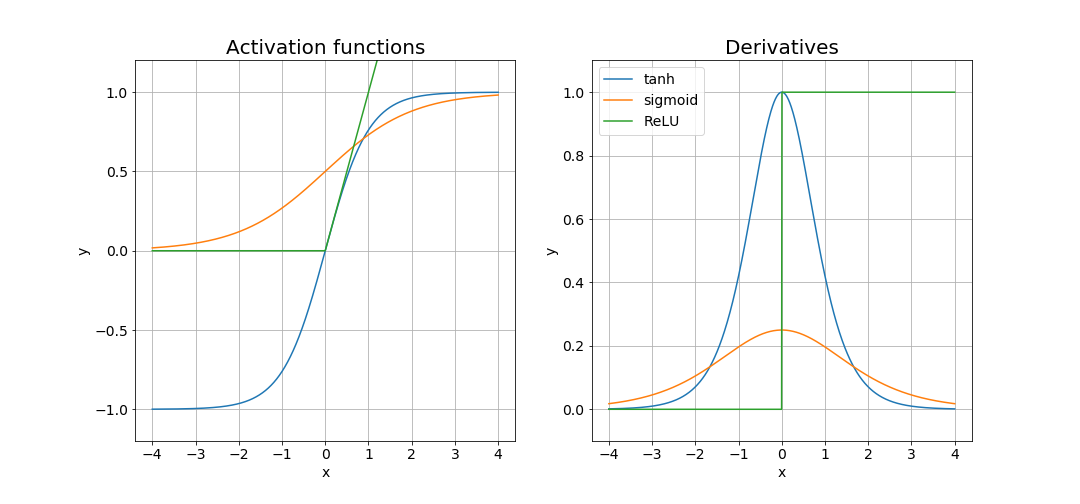
\includegraphics[scale = 0.5]{activation_functions_and_derivatives.png}
    \caption{Figure showing the shapes of activation function. Both sigmoid and tanh saturate at one, and vanish for 0 and -1 respectively. Gradient based learning doesn't learn the. ReLU doesn't have this problem with saturation.}
    \label{fig:activation_func_plus}
\end{figure}

\input{convolutional_layer}

\subsubsection{Transforming data} \label{sec:transforming_cloud_cover}
\textbf{Inverse of sigmoid is often refered to as logistic sigmoid?}
Transformation of data us useful for avoiding predicting unphysical values. As well as keeping digits from exploding.
A common approach for values in the range zero to one is using the inverse of the sigmoid function, shown in figure \ref{fig:activation_func_plus}. The transform uses values from the entire real axis $(-\infty, \infty)$. 
%\input{Chapter2_Theory/tikz/sigmoid.tikz}
Tranforming the data using sigmoid and then squazing it back between 0 and 1. 
Continous models can learn out-of-sample values. In this case it would be unphysical.

\subsection{Loss/ Metrics}  \label{sec:metrics}
In order to acquire a certain skill you need a measure determining how close you are. 
Use the sum of square or absolute values in order to not penalize point on the lower side of the line. Or not having to deal with negative distances. 
\begin{equation} \label{eq:mse}
    MSE(\hat{y},\hat{\tilde{y}}) = \frac{1}{n} \sum_{i=0}^{n-1}(y_i-\tilde{y}_i)^2
\end{equation} 

\begin{equation} \label{eq:ase}
    ASE(\hat{y},\hat{\tilde{y}}) =  \sum_{i=0}^{n-1}(y_i-\tilde{y}_i)^2
\end{equation} 

\begin{equation} \label{eq:r2}
    R^2(\hat{y}, \tilde{\hat{y}}) = 1 - \frac{\sum_{i=0}^{n - 1} (y_i - \tilde{y}_i)^2}{\sum_{i=0}^{n - 1} (y_i - \bar{y})^2}
\end{equation} 
where mean value of $\hat{y}$ is defined as $\bar{y} =  \frac{1}{n} \sum_{i=0}^{n - 1} y_i$. $R^2$ describes how much of the variation in the dataset you are able to capture with your model.

\subsection{Generalization} \label{sec:generalization}
% Move overfitting here
Finding a suitable curve for a set of points. Working with real data, noise is inevitable. In order to compensate, data is split into training and test (validation) sets. % better to call it something like generalization..?
Overall goal is to achieve the most general relation. \textit{For prediction purposes they can sometimes outperform fancier non-linear models, especially in situations with small numbers of training cases, low signal-to-noise ratio or sparse data.} \textbf{Hastie et al.} Overfitting becomes evident when you have a increase in the difference between the test- and training error. In non-mathematical terms, you have adjusted to much to the training data and where not able to find the general relation, program or "rules". See Figure \ref{fig:linreg_overfitting} 

\begin{figure}[hp]
    \centering
    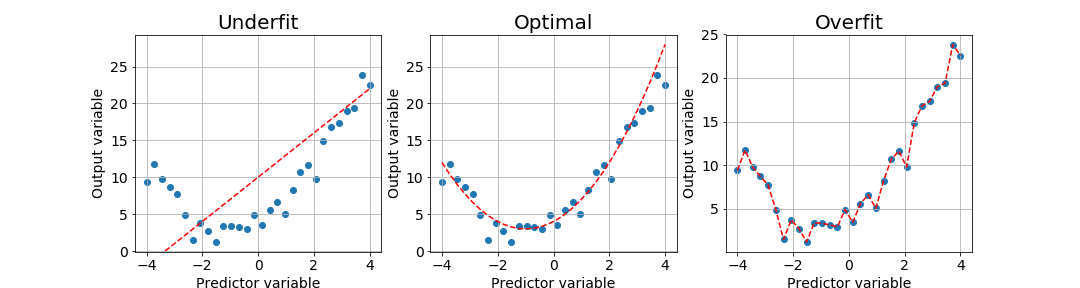
\includegraphics[scale = 0.5]{generalization.png}
    \caption{Fitting at different levels. The optimal fit is the most general one. This is applicable to many cases. For the traditional autoregressive models, the predictor variable is the true value in the previous time step. \textbf{I'll make my own figure if we decide it should be a part of my thesis.}}
    \label{fig:linreg_overfitting}
\end{figure}

Its relevant for all ML algorithms but easiest to visualize for linear regression.
\textit{Overfitting a model is a condition where a statistical model begins to describe the random error in the data rather than the relationships between variables.}

\subsection{Automatic Optimization} \label{sec:hyperparam_tuning}
Keras-tuner. Tuning hyper-parameters.
\textit{A hyperparameter is a constant parameter whose value is set before the learning process begins.}

\textbf{Explain all the params you tune. Might be beneficially with a figure. See Rune's MS-thesis.}

\textit{Learning to forget found the best accuracy when using learning rate decay.}


Although theoretically fascinating it remains to see if LSTM provide a clear practical advantage over the autoregressive models.

%%%%%%%%%%%%%%%%%%%%%%%%%%%%%%%%%%%%%%%%%%%%%%%%%%%%%%%%%%%%%%%%%%%%%%%%%%%%%%%%%%%%%%%%%%%%%

%\subsection{Neural network}
%\begin{figure}[hp]
\centering
\def\layersep{2.5cm}
\begin{tikzpicture}[shorten >=1pt,->,draw=black!50, node distance=\layersep]
    \tikzstyle{every pin edge}=[<-,shorten <=1pt]
    \tikzstyle{neuron}=[circle,fill=black!25,minimum size=17pt,inner sep=0pt]
    \tikzstyle{input neuron}=[neuron, fill=blue!50];
    \tikzstyle{output neuron}=[neuron, fill=red!50];
    \tikzstyle{hidden neuron}=[neuron, fill=green!50];
    \tikzstyle{annot} = [text width=4em, text centered]

    \node[input neuron] (I-1) at (0,-1) {}; % {$T_{2m}$};
    \node[input neuron] (I-2) at (0,-2) {}; % {$q_v$};
    \node[input neuron] (I-3) at (0,-3) {}; % {$RH$};
    \node[input neuron] (I-4) at (0,-4) {}; % {$p_s$};

    % Draw the input layer nodes
    %\foreach \name / \y in {1,...,4}
    % This is the same as writing \foreach \name / \y in {1/1,2/2,3/3,4/4}
    %    \node[input neuron, pin=left:Input \#\y] (I-\name) at (0,-\y) {};

    % Draw the hidden layer nodes
    \foreach \name / \y in {1,...,5}
        \path[yshift=0.5cm]
            node[hidden neuron] (H-\name) at (\layersep,-\y cm) {};

    % Draw the output layer node
    \node[output neuron, right of=H-2] (O) {};
    \node[output neuron, right of=H-3] (O1) {};
    \node[output neuron, right of=H-4] (O2) {};


    % Connect every node in the input layer with every node in the
    % hidden layer.
    \foreach \source in {1,...,4}
        \foreach \dest in {1,...,5}
            \path (I-\source) edge (H-\dest);

    % Connect every node in the hidden layer with the output layer
    \foreach \source in {1,...,5}
        \path (H-\source) edge (O);
        %\path (H-\source) edge (o1);
        %\path (H-\source) edge (o2);

    % Does the same thing the loop does had to do it manually tho
    \path (H-1) edge (O1);
    \path (H-2) edge (O1);
    \path (H-3) edge (O1);
    \path (H-4) edge (O1);
    \path (H-5) edge (O1);
    
    \path (H-1) edge (O2);
    \path (H-2) edge (O2);
    \path (H-3) edge (O2);
    \path (H-4) edge (O2);
    \path (H-5) edge (O2);

    % Annotate the layers
    \node[annot,above of=H-1, node distance=1cm] (hl) {Hidden layer};
    \node[annot,left of=hl] {Input layer};
    \node[annot,right of=hl] {Output layer};
\end{tikzpicture}

\caption{2-layer neural network. The connections between the layers are the weights. The input layer has four units, the hidden layer has five and the output layer has three. In total there is 35 parameters in this network (37 if \textcolor{red}{..bias is included}  we include bias). The sketch is based on the example from Skissen bygger viderer på eksempelet fra \href{http://www.texample.net/tikz/examples/neural-network/}{http://www.texample.net/tikz/examples/neural-network/}}
\label{fig:one_layer_mlp}
\end{figure}
%Figure \ref{fig:one_layer_mlp} shows a simple architecture of a neural network. This consist of four input nodes or neurons, one for each of the variables relevant for the problem at hand. This is a fully connected network, meaning that every input node has a connection/weight to the next layer. After the input data has been passed to the hidden layer (sum over the matrix multiplication of the data and weight) it goes though a activation. The activation function in neural networks introduce the non-linearity's. Without then this would be piece-wise linear functions\textbf{..?}. Figure \ref{fig:activation_one_node} illustrates the activation in one node based on the input of variables. 
%\begin{figure}[hp!]
\centering
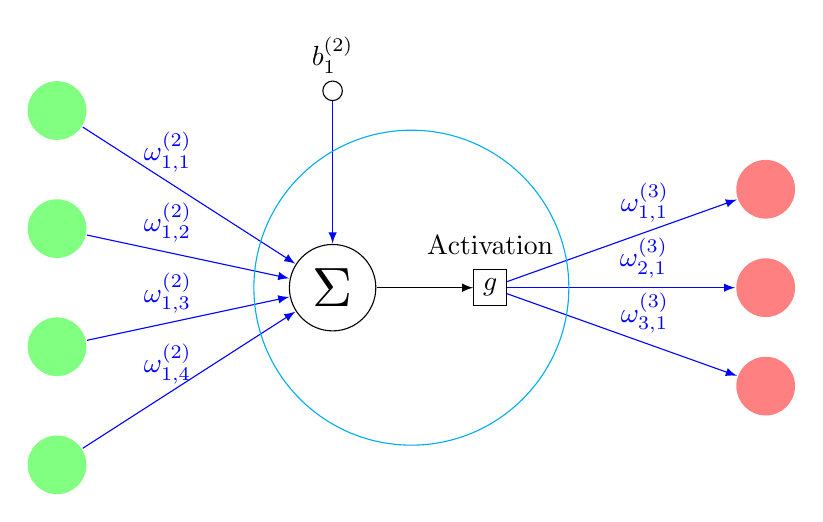
\begin{tikzpicture}[>=latex]
\path
(0,0)     node[circle,draw,scale=2,inner sep=2pt] (S) {$\Sigma$}
+(90:2.5) node[circle,draw,inner sep=2.5pt] (b) {}
          node[above=1mm] {$b_1^{(2)}$}
+(-3.5,2.25)  node[circle,scale=2.25,fill=green!50]  (x1) {} %{$T_{2m}$}
+(-3.5,0.75)  node[circle,scale=2.25,fill=green!50]  (x2) {} %{$q_v$}
+(-3.5,-0.75) node[circle,scale=2.25,fill=green!50]  (x3) {} %{$RH$}
+(-3.5,-2.25) node[circle,scale=2.25,fill=green!50]  (x4) {} %{$p_s$}
(2,0)    node[draw] (g) {$g$} node[above=3mm]{Activation}

+(3.5,1.25)  node[circle,scale=2.25,fill=red!50]  (y1) {}
+(3.5,0)  node[circle,scale=2.25,fill=red!50]  (y3) {}
+(3.5,-1.25) node[circle,scale=2.25,fill=red!50]  (y2) {};

\draw[->, black] (S)--(g);
\draw[->, blue] (b)--(S);
\draw[->, blue] (g)--(y1) node[pos=.6,above, blue]{$\omega_{1,1}^{(3)}$};
\draw[->, blue] (g)--(y2) node[pos=.6,above, blue]{$\omega_{3,1}^{(3)}$};
\draw[->, blue] (g)--(y3) node[pos=.6,above, blue]{$\omega_{2,1}^{(3)}$};

\draw[->, blue] (x1)--(S) node[pos=.4,above, blue]{$\omega_{1,1}^{(2)}$};
\draw[->, blue] (x2)--(S) node[pos=.4,above, blue]{$\omega_{1,2}^{(2)}$};
\draw[->, blue] (x3)--(S) node[pos=.4,above, blue]{$\omega_{1,3}^{(2)}$};
\draw[->, blue] (x4)--(S) node[pos=.4,above, blue]{$\omega_{1,4}^{(2)}$};
\draw[cyan] (1,0) circle(2);
\end{tikzpicture}

\caption{Computational graph showing the components participating in the activation of a neuron in the hidden layer. This example shows a 2-layer neural network with four input nodes and three output nodes. The number of nodes in the hidden layer doesn't affect the activation of the other nodes in the same layer. The sum of the weighted input and bias is passed to the activation function,
inside the hidden layers. Producing the activation of the neuron. This is again passed to the output neurons. Modified skecth based on \href{https://tex.stackexchange.com/questions/505741/architecture-neural-network-with-weights}{https://tex.stackexchange.com/questions/505741/architecture-neural-network-with-weights}. }
\label{fig:activation_one_node}
\end{figure}
%In a neural network the connections between the nodes and the biases of the nodes need to be trained. This means that the optimal first layer in three layer model, is not equal to the optimal first layer in a two layer model. 

%Three important concepts to every model. The weights, loss-function and optimiser. \textbf{neurons..?} The models is built from weights. The loss is a measure on how close you are to what you want to learn. Optimiser updates/adjust the weights in the direction of a lower loss. \textbf{Backpropagation is the learning algorithmn?} 
%\begin{equation} \label{eq:relating_cc_as_a_func}
%    tcc = f(T_{2m}, q_v, RH, sp)
%\end{equation}
%The rules I hope to achieve in this thesis is the physical relation of total cloud cover based on temperature, pressure and humidity. Like described in equation  \eqref{eq:relating_cc_as_a_func}.

%Explain Difference between a neural network used for classification and regression, is choises in cost-function and activation function in the output layer (linear for regression and softmax for classification). 


%\subsubsection{Convolution}
%Convolution is a mathematical operation where you move a filter across you two dimensional data. Here the result in one cell is the affected by its neighbours. In a convolution neural network the trained weights are the filters. 
%% kilde https://tex.stackexchange.com/questions/522118/visualizing-matrix-convolution 
\begin{figure}[hp]
    \centering
    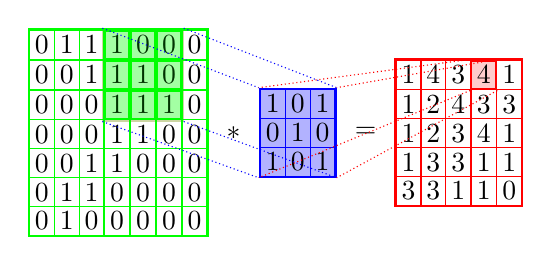
\begin{tikzpicture}[mmat/.style={matrix of math nodes,column sep=-\pgflinewidth/2,
   row sep=-\pgflinewidth/2,cells={nodes={draw,inner sep=2pt,thin}},draw=#1,thick, inner sep=0pt},
   mmat/.default=green,
   node distance=0.3em]
   
 \matrix[mmat](mat1){
         0 & 1 & 1 & |[draw=green,thick,fill=green!20,alias=1]| 1 & |[draw=green,thick,fill=green!20,alias=0]| 0 & |[draw=green,thick,fill=green!20,alias=]| 0 & 0 \\ 
         0 & 0 & 1 & |[draw=green,thick,fill=green!20,alias=1]|1 & |[draw=green,thick,fill=green!20,alias=1]|1 &|[draw=green,thick,fill=green!20,alias=0]| 0 & 0 \\ 
         0 & 0 & 0 & |[draw=green,thick,fill=green!20,alias=1]|1 &|[draw=green,thick,fill=green!20,alias=1]| 1 & |[draw=green,thick,fill=green!20,alias=1]|1 & 0 \\ 
         0 & 0 & 0 & 1 & 1 & 0 & 0 \\ 
         0 & 0 & 1 & 1 & 0 & 0 & 0 \\ 
         0 & 1 & 1 & 0 & 0 & 0 & 0 \\ 
         0 & 1 & 0 & 0 & 0 & 0 & 0 \\ 
         };
 \node[fit=(mat1-1-4)(mat1-3-6),inner sep=0pt, draw, green, thick, fill = green, opacity = 0.2](f1){};        
 
 \node[right=of mat1] (mul) {$*$};      
 \matrix[mmat=blue,fill=blue!30,right=of mul](mat2){    
     1 & 0 & 1 \\ 
     0 & 1 & 0 \\ 
     1 & 0 & 1 \\ };
 \node[right=of mat2] (eq) {$=$};       
 \matrix[mmat,right=of eq, draw = red](mat3){    
     1 & 4 & 3 & |[draw=red,thick,fill=red!20,alias=4]|4 & 1 \\ 
     1 & 2 & 4 & 3 & 3 \\ 
     1 & 2 & 3 & 4 & 1 \\ 
     1 & 3 & 3 & 1 & 1 \\ 
     3 & 3 & 1 & 1 & 0 \\ 
 };
 \foreach \Anchor in {south west,north west,south east,north east}
 {\draw[blue,densely dotted] (f1.\Anchor) -- (mat2.\Anchor); 
 \draw[red,densely dotted] (4.\Anchor) -- (mat2.\Anchor);}
 \begin{scope}[on background layer]
  \fill[red!20] (f1.north west) rectangle (f1.south east);
 \end{scope}
 
 
\end{tikzpicture}
    \caption{Diagram showing a convolutional operation. Inspired by \textbf{Cite}
    \href{https://tex.stackexchange.com/questions/522118/visualizing-matrix-convolution}{https://tex.stackexchange.com/questions/522118/visualizing-matrix-convolution}}
    \label{fig:convolution}
\end{figure}

%\input{Chapter2_Theory/tikz/lstm_cell.tikz}

%\input{Chapter2_Theory/tikz/spherical_vs_cartesian.tikz}

%\begin{figure}
%    \centering
%    \includegraphics{Chapter2_Theory/images/classification_overfitted.png}
%    \caption{Caption}
%    \label{fig:classification_overfitting}
%\end{figure}

%Climate models are implementations of physical equations and parametrizations. After some tuning they are thought to provide the answers given a state. You can read more about climate models in section \ref{sec:climate_models}. Since Hansen et. al. 1984 \textbf{siter} first attempted to estimate the acrfull{ecs}, reaserchers have been working on reducing the spread. 
%More complex models introduce other uncertainties and they have not yet been able to reduce it sufficiently \textbf{hvordan si "nok" - uten at et blir slemt}. With data available, more complex relations can be described. This requires deeper networks and the depth in deep learning refers to the number of layers. More complex models come with a higher risk of overfitting. \textbf{Kilde book Chollet}.



\section{Future work}
\begin{enumerate}
    \item Describe how to make parametrization to implement in CMIP6.
    \item Programming language in climate models vs python.
\end{enumerate}



%\section{Deep learning - ikke den ina rettet}
%acrfull{ai} is a part of our daily lives. From face recognition unlocking your phone to self driving busses in the Oslo city centre. Speech recognition, to can tell your phone what to write in your emails. Manpulating videos. Making it look like important people are saying something else than they originally did. \\ \\
%The field dates back to the fifties. When pioneers started\textit{ discussing how one could automatise tasks normally performed by humans.} Three factors determining the advances of the field; data, hardware and algorithmns. Logistic regression and Naive Bayes classifiers are examples of algorithmns that predates computers, but are still very useful to this day. Internet continuous to provide large amounts of data from Wikipedia, Flicker (tagged images) and YouTube. Advances in computational powers, such as graphical processing units, GPU's \textit{provide a environment/platform=os to learn in/on}. These where originally develop for the gaming industry, but in 2007 they realised a interface called CUDA (2007) which allows for computing \textbf{find a up to date cost and flops (floating point operations per second)}. \textbf{siter Chollet bok}


%For clarity, the deep in deep learning refer to the number of layers. Moving from shallow networks to deeper ones (more than 10) algorithmic advances in gradient propagation was needed. The main advantage of using deep neural networks is that they find their own feature representations of the given data. AI promises that if you have enough data you can find any relation. However this is not always the case, you have to add noise, non stationary system (e.g. climate) and miss-labeled data. Theorem. Data always contain noise. Using supervised learning the data might be incorrectly labelled. Human makes mistake. Earth system monitoring provides a global view of variables across meteorological systems. %\textbf{Some thing about satellite era}. These large amounts of data and the flexible nature of the neural network makes is a suitable method also in geosciences. \textbf{With enough data neural networks can serve as a universal function approximate given a suitable hyper parameter tuning and input data.} 
%The last couple of years reaserchers have been attempting to use this for wide range of problems like rainfall runoff modeling (krazerts), high-resolution weather forecasting (Rodrigues), Air quality forecasting (sun and liu), precipitaiton nowcasting (Shi et al) and \textbf{kanskje: LES} \textit{deep neural network based feature representation for weather data.} \textbf{lui et al }. \textbf{noe med forskjellig hell.} Another more comprehensive machine learning project is lead by Tapio Schneider at Caltech. Along with his team of technologist they have ambitions to create a earth system model using machine learning. With his team of from MIT and former employees of Microsoft and Google they hope to create a platform which can resolve clouds and hopefully reduce the spread in climate sensitivity. \textbf{cite Science}



%This includes activation functions, weight initialisation and optimisation schemes. I'll get back to that in section \ref{sec:intro_machine_learning}. Other advances like batch normalisation, depth wise separable convolutions attributed to the revolution of \acrshort{ai}. 
%\begin{figure}[h]
%    \centering
%    \includegraphics{Chapter1_Intro/images/Datenvolumen_D-SDA.jpg}
%    \caption{Data volume. By the continuous earth system monitoring, meteorology/ climate science have progressed toward becoming a big data science. Observations are most used for verifying climate models and quantifying the current state of climate. \href{https://www.dlr.de/eoc/en/desktopdefault.aspx/tabid-12632/22039_read-51751}{https://www.dlr.de/eoc/en/desktopdefault.aspx/tabid-12632/22039{\_}read-51751}.}
%    \label{fig:data_volum_sat}
%\end{figure}

\end{document}
